\documentclass[11pt,fleqn, openany]{book} % Default font size and left-justified equations

%%%%%%%%%%%%%%%%%%%%%%%%%%%%%%%%%%%%%%%%%
% The Legrand Orange Book
% Structural Definitions File
% Version 2.1 (26/09/2018)
%
% Original author:
% Mathias Legrand (legrand.mathias@gmail.com) with modifications by:
% Vel (vel@latextemplates.com)
% 
% This file was downloaded from:
% http://www.LaTeXTemplates.com
%
% License:
% CC BY-NC-SA 3.0 (http://creativecommons.org/licenses/by-nc-sa/3.0/)
%
%%%%%%%%%%%%%%%%%%%%%%%%%%%%%%%%%%%%%%%%%

%----------------------------------------------------------------------------------------
%	VARIOUS REQUIRED PACKAGES AND CONFIGURATIONS
%----------------------------------------------------------------------------------------

\usepackage[table]{xcolor}

\usepackage{graphicx}
\usepackage{tabularx} % Required for including pictures
\usepackage{pgf,tikz,tkz-tab,eurosym,yhmath, stmaryrd}
\usepackage{pgfplots}
\usepackage{mathrsfs}
\usetikzlibrary{patterns}
\usetikzlibrary{trees}
\graphicspath{{../../Pictures/}}
\usepackage{multicol} 


\usepackage[english]{babel} % English language/hyphenation
\usepackage{icomma}
\usepackage{enumitem} % Customize lists
\setlist{nolistsep, nosep, nolistsep} % Reduce spacing between bullet points and numbered lists

\usepackage{booktabs} % Required for nicer horizontal rules in tables

 % Required for specifying colors by name


\definecolor{ocre}{RGB}{243,102,25} % Define the orange color used for highlighting throughout the book

\usepackage{listings}

\definecolor{codegreen}{rgb}{0,0.6,0}
\definecolor{codegray}{rgb}{0.5,0.5,0.5}
\definecolor{codepurple}{rgb}{0.58,0,0.82}
\definecolor{backcolour}{rgb}{0.95,0.95,0.92}

\lstdefinestyle{mystyle}{
    backgroundcolor=\color{backcolour},   
    commentstyle=\color{codegreen},
    keywordstyle=\color{magenta},
    numberstyle=\tiny\color{codegray},
    stringstyle=\color{codepurple},
    basicstyle=\ttfamily\footnotesize,
    breakatwhitespace=false,         
    breaklines=true,                 
    captionpos=b,                    
    keepspaces=true,                 
    numbers=left,                    
    numbersep=5pt,                  
    showspaces=false,                
    showstringspaces=false,
    showtabs=false,                  
    tabsize=2
}

\lstset{style=mystyle}

%----------------------------------------------------------------------------------------
% Paramétrage XSIM
%----------------------------------------------------------------------------------------

\usepackage[no-files]{xsim}


\DeclareExerciseEnvironmentTemplate{myex}{%
    \textbf{%
      \hypertarget{ex:\ExerciseID}{\sffamily{\ensuremath{\blacktriangleright}} Exercice \GetExerciseProperty{counter} \GetExerciseProperty{subtitle} --}
      \hyperlink{sol:\ExerciseID}{Voir le corrigé}%
    }\par
}{\par\smallskip}

\DeclareExerciseEnvironmentTemplate{mysol}{%
    \textbf{%
      \hypertarget{sol:\ExerciseID}{\sffamily{\ensuremath{\blacktriangleright}} Correction \GetExerciseProperty{counter} --}
      \hyperlink{ex:\ExerciseID}{Voir l'énoncé}%
    }\par
}{\par\medskip}

\xsimsetup{
  exercise/template = myex ,
  solution/template = mysol 
}

%Collection exercices

\DeclareExerciseTagging{topic}

\xsimsetup{collect}

%----------------------------------------------------------------------------------------
% SYMBOLES
%----------------------------------------------------------------------------------------

\newcommand\imCMsym[4][\mathord]{%
  \DeclareFontFamily{U} {#2}{}
  \DeclareFontShape{U}{#2}{m}{n}{
    <-6> #25
    <6-7> #26
    <7-8> #27
    <8-9> #28
    <9-10> #29
    <10-12> #210
    <12-> #212}{}
  \DeclareSymbolFont{CM#2} {U} {#2}{m}{n}
  \DeclareMathSymbol{#4}{#1}{CM#2}{#3}
}
\newcommand\alsoimCMsym[4][\mathord]{\DeclareMathSymbol{#4}{#1}{CM#2}{#3}}

\imCMsym{cmmi}{124}{\CMjmath}

\newcommand{\Oij}{(O\,;\,\vec{\imath}\,,\, \vec{\CMjmath} )}
\newcommand{\Oijk}{(O\,;\,\vec{\imath}\,,\, \vec{\CMjmath}\,,\,\vec{k})}

\newcommand\e{\mathrm{e}}
\newcommand\R{\mathbb{R}}
\newcommand\N{\mathbb{N}}


%----------------------------------------------------------------------------------------
%	MARGINS
%----------------------------------------------------------------------------------------

\usepackage{geometry} % Required for adjusting page dimensions and margins

\geometry{
	paper=a4paper, % Paper size, change to letterpaper for US letter size
	top=3cm, % Top margin
	bottom=3cm, % Bottom margin
	left=2cm, % Left margin
	right=2cm, % Right margin
	headheight=14pt, % Header height
	footskip=1.4cm, % Space from the bottom margin to the baseline of the footer
	headsep=10pt, % Space from the top margin to the baseline of the header
	%showframe, % Uncomment to show how the type block is set on the page
}

\setlength{\parindent}{0pt}
\parskip=5pt



%----------------------------------------------------------------------------------------
%	FONTS
%----------------------------------------------------------------------------------------

\usepackage{avant} % Use the Avantgarde font for headings
\usepackage{times} % Use the Times font for headings
\usepackage{mathptmx} % Use the Adobe Times Roman as the default text font together with math symbols from the Sym­bol, Chancery and Com­puter Modern fonts

%\usepackage{microtype} % Slightly tweak font spacing for aesthetics
%\usepackage[utf8]{inputenc} % Required for including letters with accents
\usepackage[T1]{fontenc} % Use 8-bit encoding that has 256 glyphs

%----------------------------------------------------------------------------------------
%	BIBLIOGRAPHY AND INDEX
%----------------------------------------------------------------------------------------

\usepackage[style=numeric,citestyle=numeric,sorting=nyt,sortcites=true,autopunct=true,babel=hyphen,hyperref=true,abbreviate=false,backref=true,backend=biber]{biblatex}
\addbibresource{bibliography.bib} % BibTeX bibliography file
\defbibheading{bibempty}{}

\usepackage{calc} % For simpler calculation - used for spacing the index letter headings correctly
\usepackage{makeidx} % Required to make an index
\makeindex % Tells LaTeX to create the files required for indexing

%----------------------------------------------------------------------------------------
%	MAIN TABLE OF CONTENTS
%----------------------------------------------------------------------------------------

\usepackage{titletoc} % Required for manipulating the table of contents

\contentsmargin{0cm} % Removes the default margin

% Part text styling (this is mostly taken care of in the PART HEADINGS section of this file)
\titlecontents{part}
	[0cm] % Left indentation
	{\addvspace{20pt}\bfseries} % Spacing and font options for parts
	{}
	{}
	{}

% Chapter text styling
\titlecontents{chapter}
	[1.25cm] % Left indentation
	{\addvspace{12pt}\large\sffamily\bfseries} % Spacing and font options for chapters
	{\color{ocre!60}\contentslabel[\Large\thecontentslabel]{1.25cm}\color{ocre}} % Formatting of numbered sections of this type
	{\color{ocre}} % Formatting of numberless sections of this type
	{\color{ocre!60}\normalsize\;\titlerule*[.5pc]{.}\;\thecontentspage} % Formatting of the filler to the right of the heading and the page number

% Section text styling
\titlecontents{section}
	[1.25cm] % Left indentation
	{\addvspace{3pt}\sffamily\bfseries} % Spacing and font options for sections
	{\contentslabel[\thecontentslabel]{1.25cm}} % Formatting of numbered sections of this type
	{} % Formatting of numberless sections of this type
	{\hfill\color{black}\thecontentspage} % Formatting of the filler to the right of the heading and the page number

% Subsection text styling
\titlecontents{subsection}
	[1.25cm] % Left indentation
	{\addvspace{1pt}\sffamily\small} % Spacing and font options for subsections
	{\contentslabel[\thecontentslabel]{1.25cm}} % Formatting of numbered sections of this type
	{} % Formatting of numberless sections of this type
	{\ \titlerule*[.5pc]{.}\;\thecontentspage} % Formatting of the filler to the right of the heading and the page number

% Figure text styling
\titlecontents{figure}
	[1.25cm] % Left indentation
	{\addvspace{1pt}\sffamily\small} % Spacing and font options for figures
	{\thecontentslabel\hspace*{1em}} % Formatting of numbered sections of this type
	{} % Formatting of numberless sections of this type
	{\ \titlerule*[.5pc]{.}\;\thecontentspage} % Formatting of the filler to the right of the heading and the page number

% Table text styling
\titlecontents{table}
	[1.25cm] % Left indentation
	{\addvspace{1pt}\sffamily\small} % Spacing and font options for tables
	{\thecontentslabel\hspace*{1em}} % Formatting of numbered sections of this type
	{} % Formatting of numberless sections of this type
	{\ \titlerule*[.5pc]{.}\;\thecontentspage} % Formatting of the filler to the right of the heading and the page number

%----------------------------------------------------------------------------------------
%	MINI TABLE OF CONTENTS IN PART HEADS
%----------------------------------------------------------------------------------------

% Chapter text styling
\titlecontents{lchapter}
	[0em] % Left indentation
	{\addvspace{15pt}\large\sffamily\bfseries} % Spacing and font options for chapters
	{\color{ocre}\contentslabel[\Large\thecontentslabel]{1.25cm}\color{ocre}} % Chapter number
	{}  
	{\color{ocre}\normalsize\sffamily\bfseries\;\titlerule*[.5pc]{.}\;\thecontentspage} % Page number

% Section text styling
\titlecontents{lsection}
	[0em] % Left indentation
	{\sffamily\small} % Spacing and font options for sections
	{\contentslabel[\thecontentslabel]{1.25cm}} % Section number
	{}
	{}

% Subsection text styling (note these aren't shown by default, display them by searchings this file for tocdepth and reading the commented text)
\titlecontents{lsubsection}
	[.5em] % Left indentation
	{\sffamily\footnotesize} % Spacing and font options for subsections
	{\contentslabel[\thecontentslabel]{1.25cm}}
	{}
	{}

%----------------------------------------------------------------------------------------
%	HEADERS AND FOOTERS
%----------------------------------------------------------------------------------------


\usepackage{fancyhdr} % Required for header and footer configuration

\pagestyle{fancy}
\renewcommand{\chaptermark}[1]{\markboth{\sffamily\normalsize\bfseries\ \thechapter.\ #1}{}} % Chapter text font settings
\renewcommand{\sectionmark}[1]{\markright{\sffamily\normalsize\thesection\hspace{5pt}#1}{}} % Section text font settings
\fancyhf{} \fancyhead[LE,RO]{\sffamily\normalsize\thepage} % Font setting for the page number in the header
\fancyhead[LO]{\rightmark} % Print the nearest section name on the left side of odd pages
\fancyhead[RE]{\leftmark} % Print the current chapter name on the right side of even pages

\fancyfoot[L]{Jason LAPEYRONNIE}
\fancyfoot[R]{\href{http://mathoutils.fr}{http://mathoutils.fr}} % Uncomment to include a footer

\renewcommand{\headrulewidth}{0.5pt} % Thickness of the rule under the header
\renewcommand{\footrulewidth}{0.5pt} % Thickness of the rule under the header

\fancypagestyle{plain}{% Style for when a plain pagestyle is specified
	\fancyhead{}\renewcommand{\headrulewidth}{0pt}%
}

% Removes the header from odd empty pages at the end of chapters
\makeatletter
\renewcommand{\cleardoublepage}{
\clearpage\ifodd\c@page\else
\hbox{}
\vspace*{\fill}
\thispagestyle{empty}
\newpage
\fi}

%----------------------------------------------------------------------------------------
%	THEOREM STYLES
%----------------------------------------------------------------------------------------

\usepackage{amsmath,amsfonts,amssymb,amsthm} % For math equations, theorems, symbols, etc

\newcommand{\intoo}[2]{\mathopen{]}#1\,;#2\mathclose{[}}
\newcommand{\ud}{\mathop{\mathrm{{}d}}\mathopen{}}
\newcommand{\intff}[2]{\mathopen{[}#1\,;#2\mathclose{]}}
\renewcommand{\qedsymbol}{$\blacksquare$}
\newtheorem{notation}{Notation}[section]

% Boxed/framed environments
\newtheoremstyle{ocrenumbox}% Theorem style name
{0pt}% Space above
{0pt}% Space below
{\normalfont}% Body font
{}% Indent amount
{\small\bf\sffamily\color{ocre}}% Theorem head font
{\;:\;}% Punctuation after theorem head
{0.25em}% Space after theorem head
{\small\sffamily\color{ocre}\thmname{#1}\nobreakspace\thmnumber{\@ifnotempty{#1}{}\@upn{#2}}% Theorem text (e.g. Theorem 2.1)
\thmnote{\nobreakspace\the\thm@notefont\sffamily\bfseries\color{black}---\nobreakspace#3}} % Optional theorem note

\newtheoremstyle{blacknumex}% Theorem style name
{5pt}% Space above
{10pt}% Space below
{\normalfont}% Body font
{} % Indent amount
{\small\bf\sffamily}% Theorem head font
{\;:\;}% Punctuation after theorem head
{0.25em}% Space after theorem head
{\small\sffamily{\tiny\ensuremath{\blacksquare}}\nobreakspace\thmname{#1}\nobreakspace\thmnumber{\@ifnotempty{#1}{}\@upn{#2}}% Theorem text (e.g. Theorem 2.1)
\thmnote{\nobreakspace\the\thm@notefont\sffamily\bfseries---\nobreakspace#3}}% Optional theorem note

\newtheoremstyle{blacknumexo}% Theorem style name
{15pt}% Space above
{10pt}% Space below
{\normalfont}% Body font
{} % Indent amount
{\small\bf\sffamily}% Theorem head font
{}% Punctuation after theorem head
{0.5em}% Space after theorem head
{\small\sffamily{\ensuremath{\blacktriangleright}}\nobreakspace\thmname{#1}\nobreakspace\thmnumber{\@ifnotempty{#1}{}\@upn{#2}}% Theorem text (e.g. Theorem 2.1)
\thmnote{\nobreakspace\the\thm@notefont\sffamily\bfseries---\nobreakspace#3} \\}% Optional theorem note



\newtheoremstyle{blacknumbox} % Theorem style name
{0pt}% Space above
{5pt}% Space below
{}% Body font
{}% Indent amount
{\large\bf\sffamily}% Theorem head font
{\;:\;}% Punctuation after theorem head
{0.25em}% Space after theorem head
{\small\sffamily\thmname{#1}\nobreakspace\thmnumber{\@ifnotempty{#1}{}\@upn{#2}}% Theorem text (e.g. Theorem 2.1)
\thmnote{\nobreakspace\the\thm@notefont\sffamily\bfseries---\nobreakspace#3}}% Optional theorem note

% Non-boxed/non-framed environments
\newtheoremstyle{ocrenum}% Theorem style name
{5pt}% Space above
{5pt}% Space below
{\normalfont}% Body font
{}% Indent amount
{\small\bf\sffamily\color{ocre}}% Theorem head font
{\;:\;}% Punctuation after theorem head
{0.25em}% Space after theorem head
{\small\sffamily\color{ocre}\thmname{#1}\nobreakspace\thmnumber{\@ifnotempty{#1}{}\@upn{#2}}% Theorem text (e.g. Theorem 2.1)
\thmnote{\nobreakspace\the\thm@notefont\sffamily\bfseries\color{black}---\nobreakspace#3}} % Optional theorem note
\makeatother

% Defines the theorem text style for each type of theorem to one of the three styles above
\newcounter{dummy} 
\newcounter{thm}
\newcounter{correction}
\newcounter{qst}
\theoremstyle{ocrenumbox}
\newtheorem{theoremeT}[dummy]{Théorème}
\newtheorem{exerciseT}{Propriété}
\newtheorem{principeT}{Principe}
\theoremstyle{blacknumex}
\newtheorem{exampleT}{Exemple}
\theoremstyle{blacknumexo}
\newtheorem{exo}[thm]{Exercice}
\newtheorem{corr}[correction]{Correction}
\newtheorem{quest}[qst]{Question}
\theoremstyle{blacknumbox}
\newtheorem{vocabulary}{Vocabulary}[section]
\newtheorem{definitionT}{Définition}
\newtheorem{corollaryT}[dummy]{Corollary}
\theoremstyle{ocrenum}
\newtheorem{proofT}[dummy]{Démonstration}


%----------------------------------------------------------------------------------------
%	DEFINITION OF COLORED BOXES
%----------------------------------------------------------------------------------------

\RequirePackage[framemethod=default]{mdframed} % Required for creating the theorem, definition, exercise and corollary boxes

% Theorem box
\newmdenv[skipabove=7pt,
skipbelow=7pt,
backgroundcolor=black!5,
linecolor=ocre,
innerleftmargin=5pt,
innerrightmargin=5pt,
innertopmargin=10pt,
leftmargin=0cm,
rightmargin=0cm,
innerbottommargin=5pt]{tBox}

%Proposition box	  
\newmdenv[skipabove=7pt,
skipbelow=7pt,
rightline=false,
leftline=true,
topline=false,
bottomline=false,
backgroundcolor=ocre!10,
linecolor=ocre,
innerleftmargin=5pt,
innerrightmargin=5pt,
innertopmargin=10pt,
innerbottommargin=3pt,
leftmargin=0cm,
rightmargin=0cm,
linewidth=4pt]{eBox}	

% Definition box
\newmdenv[skipabove=7pt,
backgroundcolor=ocre!4,
skipbelow=7pt,
rightline=false,
leftline=true,
topline=false,
bottomline=false,
linecolor=ocre,
innerleftmargin=5pt,
innerrightmargin=5pt,
innertopmargin=10pt,
leftmargin=0cm,
rightmargin=0cm,
linewidth=4pt,
innerbottommargin=5pt]{dBox}	

% Corollary box
\newmdenv[skipabove=7pt,
skipbelow=7pt,
rightline=false,
leftline=true,
topline=false,
bottomline=false,
linecolor=gray,
backgroundcolor=black!5,
innerleftmargin=5pt,
innerrightmargin=5pt,
innertopmargin=5pt,
leftmargin=0cm,
rightmargin=0cm,
linewidth=4pt,
innerbottommargin=5pt]{cBox}

\newmdenv[skipabove=7pt,
skipbelow=7pt,
backgroundcolor=black!5,
innerleftmargin=5pt,
topline=false,
bottomline=false,
rightline=false,
leftline=false,
innerrightmargin=5pt,
innertopmargin=5pt,
leftmargin=0cm,
rightmargin=0cm,
innerbottommargin=5pt]{xBox}

% Creates an environment for each type of theorem and assigns it a theorem text style from the "Theorem Styles" section above and a colored box from above
\newenvironment{theorem}{\begin{tBox}\begin{theoremeT}}{\end{theoremeT}\end{tBox}}

\newenvironment{exo2}{\noindent \begin{exo}\item\relax \noindent \begin{eBox}\item\relax}{\end{eBox}\end{exo}}


\newenvironment{proposition}{\begin{eBox}\begin{exerciseT}}{\hfill{\color{ocre}}\end{exerciseT}\end{eBox}}		

\newenvironment{principe}{\begin{eBox}\begin{principeT}}{\hfill{\color{ocre}}\end{principeT}\end{eBox}}	
		  
\newenvironment{definition}{\begin{dBox}\begin{definitionT}}{\end{definitionT}\end{dBox}}	

\newenvironment{example}{\begin{xBox}\begin{exampleT}}{\hfill{\tiny\ensuremath{\blacksquare}}\end{exampleT}\end{xBox}}

\newenvironment{demonstration}{\begin{proofT}}{\hfill{\tiny\ensuremath{\square}}\end{proofT}}		
\newenvironment{corollary}{\begin{cBox}\begin{corollaryT}}{\end{corollaryT}\end{cBox}}	

%----------------------------------------------------------------------------------------
%	REMARK ENVIRONMENT
%----------------------------------------------------------------------------------------

\newenvironment{remark}{\par\vspace{5pt}\small % Vertical white space above the remark and smaller font size
\begin{list}{}{
\leftmargin=25pt % Indentation on the left
\rightmargin=15pt}\item\ignorespaces % Indentation on the right
\makebox[-2.5pt]{
\begin{tikzpicture}[overlay]
\node[draw=ocre!60,line width=1pt,circle,fill=ocre!25,font=\sffamily\bfseries,inner sep=2pt,outer sep=0pt] at (-15pt,0pt){\textcolor{ocre}{R}};\end{tikzpicture}} % Orange R in a circle
\advance\baselineskip -1pt}{\end{list}\vskip5pt} % Tighter line spacing and white space after remark

%----------------------------------------------------------------------------------------
%	SECTION NUMBERING IN THE MARGIN
%----------------------------------------------------------------------------------------

\makeatletter
\renewcommand{\@seccntformat}[1]{\llap{\textcolor{ocre}{\csname the#1\endcsname}\hspace{1em}}}                    
\renewcommand{\section}{\@startsection{section}{1}{\z@}
{-4ex \@plus -1ex \@minus -.4ex}
{1ex \@plus.2ex }
{\normalfont\LARGE\sffamily\bfseries}}
\renewcommand{\subsection}{\@startsection {subsection}{2}{\z@}
{-3ex \@plus -0.1ex \@minus -.4ex}
{0.5ex \@plus.2ex }
{\normalfont\sffamily\bfseries}}
\renewcommand{\subsubsection}{\@startsection {subsubsection}{3}{\z@}
{-2ex \@plus -0.1ex \@minus -.2ex}
{.2ex \@plus.2ex }
{\normalfont\small\sffamily\bfseries}}                        
\renewcommand\paragraph{\@startsection{paragraph}{4}{\z@}
{-2ex \@plus-.2ex \@minus .2ex}
{.1ex}
{\normalfont\small\sffamily\bfseries}}

%----------------------------------------------------------------------------------------
%	PART HEADINGS
%----------------------------------------------------------------------------------------

% Numbered part in the table of contents
\newcommand{\@mypartnumtocformat}[2]{%
	\setlength\fboxsep{0pt}%
	\noindent\colorbox{ocre!20}{\strut\parbox[c][.7cm]{\ecart}{\color{ocre!70}\Large\sffamily\bfseries\centering#1}}\hskip\esp\colorbox{ocre!40}{\strut\parbox[c][.7cm]{\linewidth-\ecart-\esp}{\Large\sffamily\centering#2}}%
}

% Unnumbered part in the table of contents
\newcommand{\@myparttocformat}[1]{%
	\setlength\fboxsep{0pt}%
	\noindent\colorbox{ocre!40}{\strut\parbox[c][.7cm]{\linewidth}{\Large\sffamily\centering#1}}%
}

\newlength\esp
\setlength\esp{4pt}
\newlength\ecart
\setlength\ecart{1.2cm-\esp}
\newcommand{\thepartimage}{}%
\newcommand{\partimage}[1]{\renewcommand{\thepartimage}{#1}}%
\def\@part[#1]#2{%
\ifnum \c@secnumdepth >-2\relax%
\refstepcounter{part}%
\addcontentsline{toc}{part}{\texorpdfstring{\protect\@mypartnumtocformat{\thepart}{#1}}{\partname~\thepart\ ---\ #1}}
\else%
\addcontentsline{toc}{part}{\texorpdfstring{\protect\@myparttocformat{#1}}{#1}}%
\fi%
\startcontents%
\markboth{}{}%
{\thispagestyle{empty}%
\begin{tikzpicture}[remember picture,overlay]%
\node at (current page.north west){\begin{tikzpicture}[remember picture,overlay]%	
\fill[ocre!20](0cm,0cm) rectangle (\paperwidth,-\paperheight);
\node[anchor=north] at (4cm,-3.25cm){\color{ocre!40}\fontsize{220}{100}\sffamily\bfseries\thepart}; 
\node[anchor=south east] at (\paperwidth-1cm,-\paperheight+1cm){\parbox[t][][t]{8.5cm}{
\printcontents{l}{0}{\setcounter{tocdepth}{1}}% The depth to which the Part mini table of contents displays headings; 0 for chapters only, 1 for chapters and sections and 2 for chapters, sections and subsections
}};
\node[anchor=north east] at (\paperwidth-1.5cm,-3.25cm){\parbox[t][][t]{15cm}{\strut\raggedleft\color{white}\fontsize{30}{30}\sffamily\bfseries#2}};
\end{tikzpicture}};
\end{tikzpicture}}%
\@endpart}
\def\@spart#1{%
\startcontents%
\phantomsection
{\thispagestyle{empty}%
\begin{tikzpicture}[remember picture,overlay]%
\node at (current page.north west){\begin{tikzpicture}[remember picture,overlay]%	
\fill[ocre!20](0cm,0cm) rectangle (\paperwidth,-\paperheight);
\node[anchor=north east] at (\paperwidth-1.5cm,-3.25cm){\parbox[t][][t]{15cm}{\strut\raggedleft\color{white}\fontsize{30}{30}\sffamily\bfseries#1}};
\end{tikzpicture}};
\end{tikzpicture}}
\addcontentsline{toc}{part}{\texorpdfstring{%
\setlength\fboxsep{0pt}%
\noindent\protect\colorbox{ocre!40}{\strut\protect\parbox[c][.7cm]{\linewidth}{\Large\sffamily\protect\centering #1\quad\mbox{}}}}{#1}}%
\@endpart}
\def\@endpart{\vfil\newpage
\if@twoside
\if@openright
\null
\thispagestyle{empty}%
\newpage
\fi
\fi
\if@tempswa
\twocolumn
\fi}

%----------------------------------------------------------------------------------------
%	CHAPTER HEADINGS
%----------------------------------------------------------------------------------------

% A switch to conditionally include a picture, implemented by Christian Hupfer
\newif\ifusechapterimage
\usechapterimagetrue
\newcommand{\thechapterimage}{}%
\newcommand{\chapterimage}[1]{\ifusechapterimage\renewcommand{\thechapterimage}{#1}\fi}%
\newcommand{\autodot}{.}
\def\@makechapterhead#1{%
{\parindent \z@ \raggedright \normalfont
\ifnum \c@secnumdepth >\m@ne
\if@mainmatter
\begin{tikzpicture}[remember picture,overlay]
\node at (current page.north west)
{\begin{tikzpicture}[remember picture,overlay]
\node[anchor=north west,inner sep=0pt] at (0,0) {\ifusechapterimage\includegraphics[width=\paperwidth]{\thechapterimage}\fi};
\draw[anchor=west] (\Gm@lmargin,-3cm) node [line width=2pt,rounded corners=15pt,draw=ocre,fill=white,fill opacity=0.5,inner sep=15pt]{\strut\makebox[22cm]{}};
\draw[anchor=west] (\Gm@lmargin+.3cm,-3cm) node {\huge\sffamily\bfseries\color{black}\thechapter\autodot~#1\strut};
\end{tikzpicture}};
\end{tikzpicture}
\else
\begin{tikzpicture}[remember picture,overlay]
\node at (current page.north west)
{\begin{tikzpicture}[remember picture,overlay]
\node[anchor=north west,inner sep=0pt] at (0,0) {\ifusechapterimage\includegraphics[width=\paperwidth]{\thechapterimage}\fi};
\draw[anchor=west] (\Gm@lmargin,-3cm) node [line width=2pt,rounded corners=15pt,draw=ocre,fill=white,fill opacity=0.5,inner sep=15pt]{\strut\makebox[22cm]{}};
\draw[anchor=west] (\Gm@lmargin+.3cm,-3cm) node {\huge\sffamily\bfseries\color{black}#1\strut};
\end{tikzpicture}};
\end{tikzpicture}
\fi\fi\par\vspace*{50\p@}}}

%-------------------------------------------

\def\@makeschapterhead#1{%
\begin{tikzpicture}[remember picture,overlay]
\node at (current page.north west)
{\begin{tikzpicture}[remember picture,overlay]
\node[anchor=north west,inner sep=0pt] at (0,0) {\ifusechapterimage\includegraphics[width=\paperwidth]{\thechapterimage}\fi};
\draw[anchor=west] (\Gm@lmargin,-3cm) node [line width=2pt,rounded corners=15pt,draw=ocre,fill=white,fill opacity=0.5,inner sep=15pt]{\strut\makebox[22cm]{}};
\draw[anchor=west] (\Gm@lmargin+.3cm,-3cm) node {\huge\sffamily\bfseries\color{black}#1\strut};
\end{tikzpicture}};
\end{tikzpicture}
\par\vspace*{50\p@}}
\makeatother

%----------------------------------------------------------------------------------------
%	LINKS
%----------------------------------------------------------------------------------------

\usepackage{hyperref}
\hypersetup{hidelinks,backref=true,pagebackref=true,hyperindex=true,colorlinks=false,breaklinks=true,urlcolor=ocre,bookmarks=true,bookmarksopen=false}

\usepackage{bookmark}
\bookmarksetup{
open,
numbered,
addtohook={%
\ifnum\bookmarkget{level}=0 % chapter
\bookmarksetup{bold}%
\fi
\ifnum\bookmarkget{level}=-1 % part
\bookmarksetup{color=ocre,bold}%
\fi
}
}

\renewcommand*\thesection{\arabic{section}}

\newcommand*{\coord}[3]{% 
  \ensuremath{\overrightarrow{#1}\, 
    \begin{pmatrix} 
      #2\\ 
      #3 
    \end{pmatrix}}}
    
  \newcommand*{\coordb}[2]{% 
  \ensuremath{ 
    \begin{pmatrix} 
      #1\\ 
      #2 
    \end{pmatrix}}}

\newcommand*{\coorde}[4]{% 
  \renewcommand{\arraystretch}{1}\ensuremath{\overrightarrow{#1}\, 
    \begin{pmatrix} 
      #2\\ 
      #3 \\
      #4
    \end{pmatrix}}}    
  \newcommand*{\coordbe}[3]{% 
 \renewcommand{\arraystretch}{1} \ensuremath{ 
    \begin{pmatrix} 
      #1\\ 
      #2 \\
      #3
    \end{pmatrix}}}  
    
\newcommand{\Card}{\mathrm{Card}}




\begin{document}

\chapterimage{../../Pictures/background}


\chapter{Cours : Primitives et équations différentielles}


\section{Notion d'équation différentielle}

\begin{definition}[Équation différentielle]Une équation différentielle est une équation dont l'inconnue est une fonction notée $y$ et qui fait intervenir les dérivées de cette fonction.\end{definition}

\begin{example}On considère la fonction $f$ définie pour tout réel $x$ par $f(x)=\e^{4x-2}$. 

$f$ est solution de l'équation différentielle $y'=4y$. 

En effet, $f$ est dérivable sur $\mathbb{R}$ et pour tout réel $x$, $f'(x)=4\e^{4x-2}$, c'est-à-dire $f'(x)=4f(x)$.\end{example}

\begin{example}On considère la fonction $f$ définie pour tout réel $x$ par $f(x)=\ln(1+\e^x)\e^{-x}$. 

$f$ est solution de l'équation différentielle $y'+y=\dfrac{1}{1+\e^x}$. En effet :

\begin{itemize}
\item Pour tout réel $x$, on pose $u(x)=\ln(1+\e^x)$. $u$ est définie et dérivable sur $\mathbb{R}$ et pour tout réel $x$, \[u'(x)=\dfrac{\e^x}{1+\e^x}.\]
\item Pour tout réel $x$, on pose $v(x)=\e^{-x}$. $v$ est dérivable sur $\mathbb{R}$ et pour tout réel $x$, $v'(x)=-\e^{-x}$.
\end{itemize}
Ainsi, $f$ est dérivable sur $\mathbb{R}$ et pour tout réel $x$,
\[f'(x)=\dfrac{\e^x}{1+\e^x}\times \e^{-x}+\ln(1+\e^x)\times(-\e^{-x})=\dfrac{1}{1+\e^x}-\ln(1+\e^x)\e^{-x}.\]
Ainsi, pour tout réel $x$,
\[f'(x)+f(x)=\dfrac{1}{1+\e^x}-\ln(1+\e^x)\e^{-x}+\ln(1+\e^x)\e^{-x}=\dfrac{1}{1+\e^x}.\]
$f$ est donc bien solution de l'équation différentielle $y'+y=\dfrac{1}{1+\e^x}$.\end{example}


\section{Primitive d'une fonction continue}



\begin{definition}Soit $f$ une fonction définie et continue sur un intervalle $I$ et $F$ une fonction dérivable sur cet intervalle. On dit que $F$ est une \textit{primitive} de $f$ sur $I$ si $F'=f$. 

Autrement dit, $F$ est solution de l'équation différentielle $y'=f$.\end{definition}


\begin{example} Pour tout réel $x$, on pose $f(x)=6x^2+4x+3$ et $F(x)=2x^3+2x^2+3x-7$. On a bien pour tout réel $x$, $F'(x)=f(x)$. $F$ est une primitive de $f$ sur $\mathbb{R}$.\end{example}



\begin{theorem}Toute fonction continue sur un intervalle $I$ admet des primitives.\end{theorem}

Ce résultat sera démontré (en partie) dans un prochain chapitre. Patience !

\begin{proposition}Soit $f$ une fonction continue sur un intervalle $I$, $F_1$ et $F_2$ deux primitives de $f$ sur $I$. 

Alors $F_1-F_2$ est constante : deux primitives d'une même fonction continue sur un intervalle différent d'une constante.\end{proposition}

\begin{demonstration} Soit $F_1$ et $F_2$ deux primitives de $f$ sur $I$.
$F_1-F_2$ est dérivable sur $I$ comme différence de fonctions dérivables sur $I$. De plus, pour tout réel $x$ dans $I$
\[ (F_1-F_2)'(x)=F_1'(x)-F_2'(x)=f(x)-f(x)=0.\]
Ainsi, $F_1-F_2$ est de dérivée nulle sur l'intervalle $I$, $F_1-F_2$ est donc constante sur $I$.\end{demonstration}

\begin{proposition}Soit $I$ un intervalle, $x_0\in I$, $y_0 \in \mathbb{R}$ et $f$ une fonction continue sur $I$. Il existe une unique primitive $F$ de $f$ sur $I$ tel que $F(x_0)=y_0$.

L'équation différentielle $y'=f$ ayant pour condition initiale $y(x_0)=y_0$ possède une unique solution.\end{proposition}


\begin{example} Pour tout réel $x$, on pose $f(x)=\dfrac{2x}{x^2+1}$ et $F(x)=\ln(x^2+1)$. 

$F$ est une primitive de $f$ sur $\mathbb{R}$. En effet, pour tout réel $x$, $F'(x)=f(x)$.

On cherche alors l'unique primitive $F_0$ de $f$ qui vaut 5 en 0. Puisque toutes les primitives d'une fonction diffèrent seulement d'une constante, il existe un réel $c$ tel que $F_0=F+c$ et donc, pour tout réel $x$, \[F_0(x)=\ln(x^2+1)+c.\] 

Puisque $F_0(0)=5$, on a alors $\ln(0^2+1)+c=5$, soit $c=5$. Pour tout réel $x$, on a donc \[F_0(x)=\ln(x^2+1)+5.\]\vspace{-0.5cm}\end{example}



\begin{proposition}Primitives usuelles
\vskip10pt
\renewcommand{\arraystretch}{2}
\begin{tabularx}{\linewidth}{|X|X|X|}

\hline
Fonction $f$ & \textbf{UNE} Primitive $F$ & Intervalle $I$ \\
\hline
$x \mapsto x^n$, $n\in \mathbb{N}$ & $x\mapsto \dfrac{x^{n+1}}{n+1}$ & $\mathbb{R}$ \\
\hline
$x \mapsto \dfrac{1}{x^n}$, $n\in \mathbb{N}\setminus\{0;1\}$ & $x\mapsto -\dfrac{1}{(n-1)x^{n-1}}$ & $]-\infty;0[$ et $]0;+\infty[$ \\
\hline
$x\mapsto \dfrac{1}{\sqrt{x}}$ & $2\sqrt{x}$ & $]0;+\infty[$ \\
\hline
$x \mapsto \e^{ax+b}$, $a\in \mathbb{R}^*$, $b\in \mathbb{R}$ & $x\mapsto \dfrac{\e^{ax+b}}{a}$ & $\mathbb{R}$ \\
\hline
$x \mapsto \dfrac{1}{x}$ & $x\mapsto \ln(x)$ & $]0;+\infty[$ \\
\hline
\end{tabularx}\end{proposition}

Le conseil de la leçon : Une fois que vous avez détermine une primitive, dérivez-la ! Vous devez obtenir la fonction de départ. Il est bien plus facile de dériver que de primitiver.

\newpage
\begin{proposition}Soit $f$ et $g$ deux fonctions continues sur un intervalle $I$, $\lambda$, $F$ une primitive de $f$ et $G$ une primitive de $g$. Alors,
\begin{itemize}
\item $F+G$ est une primitive de $f+g$ ;
\item $\lambda\,F$ est une primitive de $\lambda\,f$.
\end{itemize}\end{proposition}

\begin{example}Une primitive de la fonction $f:x\mapsto \e^{2x-1}+5x^2+\dfrac{3}{x^2}$ sur $I=]0;+\infty[$ est la fonction
\[F:x\mapsto \dfrac{\e^{2x-1}}{2}+\dfrac{5}{3}x^3-\dfrac{3}{x}.\]\end{example}



\begin{proposition}L'essentiel : Soit $f$ une fonction dérivable sur un intervalle $I$ et $g$ une fonction dérivable sur un intervalle $J$ telle que pour tout réel $x\in J$, $g(x)\in I$.

$f \circ g$ est une primitive de $g' \times (f' \circ g)$ sur $J$.\end{proposition}

Certaines "formes" de fonction sont à reconnaître pour en calculer les primitives. 

\begin{itemize}
\item Une primitive d'une fonction de la forme $-\dfrac{u'}{u^2}$ où $u$ est une fonction qui ne s'annule pas est $\dfrac{1}{u}$.
\vskip10pt
\item Une primitive d'une fonction de la forme $\dfrac{u'}{2\sqrt{u}}$ où $u$ est une fonction strictement positive est $\sqrt{u}$.
\vskip10pt
\item Une primitive d'une fonction de la forme $u'\e^u$ est $\e^u$.
\vskip10pt
\item Une primitive d'une fonction de la forme $\dfrac{u'}{u}$ où $u$ est une fonction strictement positive est $\ln(u)$.
\end{itemize}


\begin{example} Pour tout réel $x$, on pose $f(x)=(2x+1)\e^{x^2+x-2}$.

Posons, pour tout réel $x$, $u(x)=x^2+x-2$. On remarque alors que $f(x)=u'(x) \times \e^{u(x)}$.

Une primitive de $f$ est donc la fonction $F$ définie pour tout réel $x$ par $F(x)=\e^{u(x)}=\e^{x^2+x-2}$.\end{example}

\begin{example}Pour tout réel $x$, on pose $f(x)=\dfrac{2\e^{2x}}{1+\e^{2x}}$. Posons, pour tout réel $x$, $u(x)=1+\e^{2x}$. 

Pour tout réel $x$, $u(x)>0$. Par ailleurs, on remarque alors que pour tout réel $x$, $f(x)=\dfrac{u'(x)}{u(x)}$. 

Une primitive de $f$ est donc la fonction $F$ définie pour tout réel $x$, par $F(x)=\ln(u(x))=\ln(1+\e^{2x})$.\end{example}

Malheureusement, certaines fonctions n'admettent pas de primitive pouvant être exprimées à l'aide de fonctions usuelles : il s'agit là d'un théorème démontré par Liouville dans les années 1830.

L'exemple le plus notable est la fonction $x\mapsto \e^{-x^2}$, très utilisée en probabilités et dont les applications dans d'autres domaines se comptent par centaines (citons ainsi la balistique, l'évaluation du quotient intellectuel, le traitement du signal,  le cours de la bourse...).

\section{Equation différentielle  du premier ordre}

\subsection{Equations différentielles homogènes $y'+ay=0$}

\begin{definition}Soit $a$ un réel. L'équation $y'+ay=0$ ayant pour inconnue une fonction dérivable $y$ sur $\mathbb{R}$ s'appelle "équation différentielle \textbf{homogène} du premier ordre, à coefficients constants".\end{definition}

\begin{proposition}Soit $a$ un réel.

Les solutions l'équation $y'+ay=0$ sont les fonctions $f$ définies pour tout réel $x$ par $f(x)=C\e^{-ax}$ où $C$ est un réel quelconque.

De plus, pour tous réels $x_0$ et $y_0$, il existe une unique solution $f_0$ de cette équation différentielle telle que $f(x_0)=y_0$.\end{proposition}

\begin{demonstration} Soit $C$ un réel. Pour tout réel $x$, on pose alors $f(x)=C\e^{-ax}$. $f$ est dérivable sur $\mathbb{R}$ et pour tout réel $x$, $f'(x)=-a\times C\e^{-ax}=-af(x)$. Ainsi, pour tout réel $x$, \[f'(x)+af(x)=-af(x)+af(x)=0.\] $f$ est donc bien solution de l'équation différentielle $y'+ay=0$.

Réciproquement, soit $f$ une solution de l'équation $y'+ay=0$. On a alors, pour tout réel $x$, $f'(x)+a\,f(x)=0$.

Pour tout réel $x$, posons alors $g(x)=f(x)\e^{ax}$. $g$ est dérivable comme produit de fonctions dérivables et, pour tout réel $x$,
\[g'(x)=f'(x)\e^{ax}+a\,f(x) \e^{ax}=\e^{ax}(f'(x)+af(x))=0.\]
Ainsi, $g$ est constante : il existe un réel $C$ telle que, pour tout réel $x$, $g(x)=C$, c'est-à-dire $f(x)\e^{ax}=C$ et donc $f(x)=C\e^{-ax}$.\end{demonstration}

\begin{example} Les solutions de l'équation $y'-2y=0$ sont les fonctions $f:x\mapsto C\e^{2x}$ où $C$ est un réel.

Cherchons l'unique solution $f_0$ de cette équation telle que $f_0(3)=1$. Soit $C$ le réel tel que, pour tout réel $x$, $f_0(x)=C\e^{2x}$.

On a alors $f_0(3)=C\e^{6}$ d'une part et $f_0(3)=1$ d'autre part. Ainsi, $C=\dfrac{1}{\e^6}=\e^{-6}$. 

Finalement, pour tout réel $x$, on a $f_0(x)=\e^{-6}\e^{2x}=\e^{2x-6}$.\end{example}

Ce théorème signifie que si l'on regarde l'ensemble des courbes des fonctions solutions de l'équation $y'=ay$ et que l'on s'intéresse à un point du plan, il existe une unique courbe qui passe par ce point. En particulier, toute fonction solution qui s'annule n'est autre que la fonction nulle.

\begin{center}
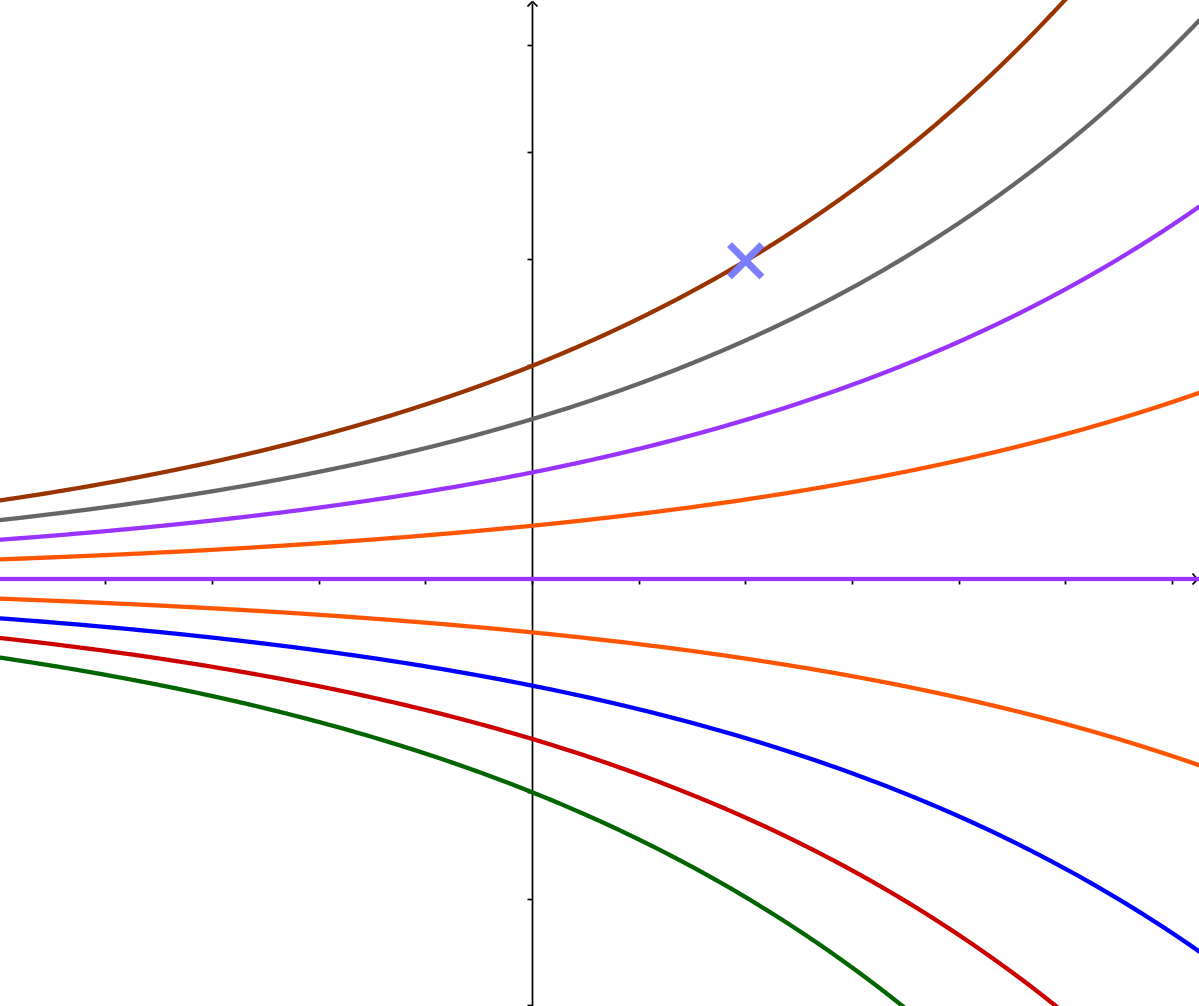
\includegraphics[scale=1.2]{equadiff}
\end{center}

\subsection{Equation différentielle $y'+ay=b$, avec $b$ réel}

\begin{definition} Soit $a$ et $b$ deux réels. L'équation $y'+ay=b$ ayant pour inconnue une fonction $y$ dérivable sur $\mathbb{R}$ s'appelle  "équation différentielle du premier ordre, à coefficients constants et à second membre constant".\end{definition}

\begin{proposition}Soit $a$ et $b$ deux réels.

Les solutions de l'équation différentielle $y'+ay=b$ sont les fonctions $f$ définies pour tout réel $x$ par $f(x)=C\e^{-ax}+\dfrac{b}{a}$ où $C$ est un réel quelconque.

De plus, pour tous réels $x_0$ et $y_0$, il existe une unique solution $f_0$ de cette équation telle que $f_0(x_0)=y_0$.\end{proposition}

\begin{demonstration} Cherchons tout d'abord une solution constante $\varphi$ à cette équation. Soit $k$ le réel tel que pour tout réel $x$, $\varphi (x)=k$. $\varphi$ est dérivable sur $\mathbb{R}$ et pour tout réel $x$, $\varphi '(x)=0$.

Puisque $\varphi$ est solution de l'équation $y'+ay=b$, on a alors $ak=b$ c'est-à-dire $k=\dfrac{b}{a}$.

Soit maintenant $f$ une fonction dérivable sur $\mathbb{R}$.

$f$ est solution de l'équation différentielle $y'+ay=b$ si et seulement si $f'+af=b$. Or, $\varphi$ étant également une solution de cette équation, on a donc $b=\varphi'+a\varphi$.

Ainsi, $f$ est solution de l'équation différentielle $y'+ay=b$ si et seulement si $f'+af=\varphi+a\varphi '$, ce qui équivaut à $f'-\varphi'+a(f-\varphi)=0$, ou encore $(f-\varphi)'+a(f-\varphi)=0$.

Ainsi, $f$ est solution de l'équation différentielle $y'+ay=b$ si et seulement si $f-\varphi$ est solution de l'équation différentielle homogène $y'+ay=0$.

Il existe donc un réel $C$ tel que, pour tout réel $x$, $(f-\varphi)(x)=C\e^{-ax}$.

 Ainsi, pour tout réel $x$, $f(x)=C\e^{-ax}+\varphi(x)=C\e^{-ax}+\dfrac{b}{a}$.

\end{demonstration}



\begin{example} On cherche à résoudre l'équation $y'-5y=-2$ .

\begin{itemize}
\item On détermine les solutions de l'équation homogène associée $y'-5y=0$. 

Ce sont les fonctions $x\mapsto C\e^{5x}$ où $C$ est un réel.
\item On cherche une solution constante (égale à $k$) à l'équation de départ $y'-5y=-2$. 

La dérivée d'une fonction constante étant nulle, on a alors $-5k=-2$ et donc $k=\dfrac{2}{5}$.

\item Les fonctions solutions de l'équation $y'=5y-2$ sont donc les fonctions $f$ définies pour tout réel $x$ par $f(x)=C\e^{-5x}+\dfrac{2}{5}$ où $C$ est un réel.
\end{itemize}

On souhaite déterminer l'unique solution $f_0$ de cette équation telle que $f_0(7)=12$. Soit $C$ le réel tel que, pour tout réel $x$, $f_0(x)=C\e^{-5x}+\dfrac{2}{5}$.

On a alors $f_0(7)=C\e^{-35}+\dfrac{2}{5}=12$ et donc $C=\dfrac{58}{5}\e^{+35}$. Ainsi, pour tout réel $x$, $f_0(x)=\dfrac{58}{5}\e^{-5x+35}+\dfrac{2}{5}$.\end{example}


\begin{proposition}[Formule magique] Pour résoudre une équation du type $y'+ay=b$...
\begin{center}
\textbf{SOLUTION GÉNÉRALE = SOLUTION HOMOGÈNE + SOLUTION CONSTANTE}
\end{center}\vspace{-0.5cm}\end{proposition}


\subsection{Equation différentielle $y'+ay=g$, où $g$ est une fonction}

\begin{definition}Soit $a$ un réel non nul et $g$ une fonction définie sur $\mathbb{R}$. L'équation $y'=ay+g$ s'appelle "équation différentielle linéaire du premier ordre avec second membre".\end{definition}

\begin{proposition}Soit $a$ un réel non nul et $g$ une fonction définie sur $\mathbb{R}$. 

Soit $\varphi$ une solution particulière de cette équation. Alors $f$ est solution de l'équation $y'+ay=g$ si et seulement si $f-\varphi$ est solution de l'équation homogène associée $y'+ay=0$.

Autrement dit, toute solution de l'équation $y'+ay=g$ est de la forme $f+\varphi$, où $f$ est solution de l'équation $y'+ay=0$ et $\varphi$ est \textbf{UNE} solution de l'équation $y'+ay=g$.\end{proposition}

\begin{demonstration}La démonstration est en tout point semblable à celle qui a conduit à l'ensemble des fonctions solutions de l'équation $y'+ay=b$. Faisons-la donc à nouveau. Soit $f$ une fonction dérivable sur $\mathbb{R}$.

$f$ est solution de l'équation différentielle $y'+ay=g$ si et seulement si $f'+af=b$. Or, $\varphi$ étant également une solution de cette équation, on a donc $g=\varphi'+a\varphi$.

Ainsi, $f$ est solution de l'équation différentielle $y'+ay=g$ si et seulement si $f'+af=\varphi+a\varphi '$, ce qui équivaut à $f'-\varphi'+a(f-\varphi)=0$, ou encore $(f-\varphi)'+a(f-\varphi)=0$.

Ainsi, $f$ est solution de l'équation différentielle $y'+ay=g$ si et seulement si $f-\varphi$ est solution de l'équation différentielle homogène $y'+ay=0$.

Il existe donc un réel $C$ tel que, pour tout réel $x$, $(f-\varphi)(x)=C\e^{-ax}$ et donc $f(x)=C\e^{-ax}+\varphi(x)$.\end{demonstration}

\begin{example} On considère l'équation différentielle $y'-2y=-6x^2+13$.
\begin{itemize}
\item Les solutions de l'équation homogène associée $y'-2y=0$ sont les fonctions $x\mapsto C\e^{2x}$ où $C\in\mathbb{R}$.
\item La fonction $\varphi:x\mapsto 3x^2+3x-5$ est solution de l'équation différentielle $y'-2y=-6x^2+13$. En effet, $\varphi$ est dérivable et pour tout réel $x$, 
\[\varphi'(x)-2\varphi(x)+6x^2-13=6x+3-2(3x^2+3x-5)+6x^2-13=0.\]
\end{itemize}
Ainsi, l'ensemble des solutions de l'équation différentielle $y'-2y=-6x^2+13$ sont les fonctions $f$ définies pour tout réel $x$ par $f(x)=C\e^{2x}+3x^2+3x-5$, où $C$ est un réel.\end{example}

\begin{proposition}[Formule magique] Pour résoudre une équation du type $y'+ay+g$...
\begin{center}
\textbf{SOLUTION GÉNÉRALE = SOLUTION HOMOGÈNE + SOLUTION PARTICULIÈRE}
\end{center}\vspace{-0.5cm}\end{proposition}


Il existe de nombreux types d'équations différentielles : linéaires, quadratiques, d'ordre divers... Et parmi toutes celles-ci, il en existe peu que l'on sait résoudre.

On compte par exemple les équations de Navier-Stokes qui décrivent les mouvements des fluides newtoniens. Il s'agit d'équation dites "aux dérivées partielles". Les fonctions en jeu utilisent en effet plusieurs variables (de temps et d'espace en l'occurrence) et on dérive alors selon l'une ou l'autre des variables.

Ces équations sont particulières puisque depuis l'an 2000, leur résolution est mise à prix : quiconque permettra une avancée significative dans leur étude recevra, en plus d'un certain prestige auprès de la communauté mathématique, la coquette somme d'un million de dollars. 

6 autres problèmes ont été mis à pris par l'Institut Clay cette même année. Depuis, un seul d'entre eux a été résolu.


\chapter{Exercices}


\section*{Notion d'équation différentielle}

\begin{exercise}Montrer que $f:x \mapsto \e^{3x}+1$ est solution de l'équation différentielle $y'=3y-3$.\end{exercise}

\begin{solution}

Pour tout réel \(x\), \(f'(x)=3\e^{3x}\) et \(3f(x)-3=3(\e^{3x}+1)-3=3\e^{3x}+3-3=3\e^{3x}\).

Ainsi, pour tout réel \(x\), \(f'(x)=3f(x)-3\). \(f\) est donc solution de l'équation différentielle \(y'=3y-3\). \end{solution}



\begin{exercise}Montrer que $f:x\mapsto \dfrac{1}{1+x}$ est solution de l'équation différentielle $(1+x)y'+y=0$ sur $]-1;+\infty[$.\end{exercise}

\begin{solution}

Pour tout réel \(x\neq -1\), \(f'(x)=-\dfrac{1}{(1+x)^2}\) et donc $(1+x)f'(x)+f(x)=(1+x)\times \left(-\dfrac{1}{(1+x)^2}\right)=0$.

\(f\) est solution de l'équation différentielle \((1+x)y'+y=0\).

 \end{solution}
 
 

\begin{exercise}Montrer que $f:x \mapsto \dfrac{1}{1+\e^{-x}}$ est solution de l'équation différentielle $y'=y(1-y)$.\end{exercise}

\begin{solution}

Pour tout réel \(x\), on pose \(f(x)=\dfrac{1}{1+\e^{-x}}\). \(f\) est dérivable sur \(\mathbb{R}\) et pour tout réel \(x\), \(f'(x)=\dfrac{\e^{-x}}{(1+\e^{-x})^2}\). 

De plus, $f(x) \times (1-f(x)) = \dfrac{1}{1+\e^{-x}} \times \left(1-\dfrac{1}{1+\e^{-x}}\right)=\dfrac{\e^{-x}}{(1+\e^{-x})^2}=f'(x)$.

 \(f\) est bien solution de l'équation différentielle \(y'=y(1-y)\).
\end{solution}



\begin{exercise}Soit $\lambda$ et $\mu$ des réels. Montrer que $f:x\mapsto (\lambda x + \mu)\e^{x}$ est solution de l'équation différentielle $y''-2y'+y=0$.\end{exercise}

\begin{solution}

Pour tout réel \(x\), $f'(x)= \lambda \e^x + (\lambda x + \mu) \e^x = (\lambda x + \lambda + \mu) \e^x$
et $f^{\prime\prime}(x)=\lambda \e^x + (\lambda x + \lambda + \mu) \e^x = (\lambda x + 2\lambda + \mu) \e^x$.

Ainsi, pour tout réel \(x\),
\[\begin{array}{rcl}f^{\prime\prime}(x)-2f'(x)+f(x)&=&(\lambda x + 2\lambda + \mu) \e^x - 2 (\lambda x + \lambda + \mu) \e^x + (\lambda x + \mu)\e^{x} \\ &=& (\lambda x - 2 \lambda x + \lambda x +2 \lambda + \mu -2 \lambda - 2 \mu + \mu)\e^x \\&=&0\end{array}\]

\(f\) est bien solution de l'équation différentielle \(y^{\prime\prime}-2y'+y=0\).

\end{solution}



\section*{Primitives}

\begin{exercise}[subtitle={(Centres étrangers 2023)}]On considère une fonction $h$ définie et continue sur $\mathbb{R}$ dont le tableau de variations est le suivant.

\begin{center}
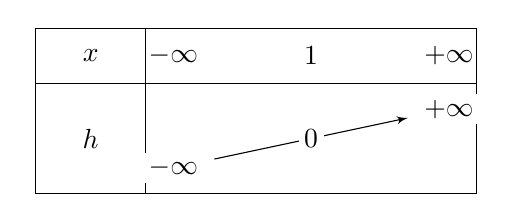
\begin{tikzpicture}[scale=0.7]
   \tkzTabInit[espcl=2.5]{$x$ / 1, $h$/2}{$-\infty$, $1$ ,$+\infty$}
      \tkzTabVar{ -/$-\infty$, R, +/$+\infty$}
      \tkzTabIma{1}{3}{2}{0}
\end{tikzpicture}
\end{center}
On note $H$ la primitive de $h$ définie sur $\mathbb{R}$ qui s'annule en 0. Quelle propriété est vérifiée par $H$ ?

\begin{minipage}{0.45\linewidth}
\textbf{a.} $H$ est positive sur $]-\infty ;0]$. \\
\textbf{b.} $H$ est croissante sur $]-\infty ;1]$.
\end{minipage}\hfill \begin{minipage}{0.45\linewidth}
\textbf{c.} $H$ est négative sur $]-\infty ;1]$. \\
\textbf{d.} $H$ est croissante sur $\mathbb{R}$.
\end{minipage}
\end{exercise}

\begin{solution}$h$ est la dérivée de $H$. Or, $h$ est négative sur $]-\infty ;0]$  : $H$ est donc décroissante sur cet intervalle. Ainsi, pour tout $x<0$, $H(x)>H(0)$. Or, $H(0)=0$. Ainsi, pour tout $x<0$, $H(x)>0$ : $H$ est positive sur $]-\infty ;0]$.\end{solution}



\begin{exercise}Montrer que la fonction $f:x\mapsto x\ln(x)-x$ est une primitive de $\ln$ sur $]0;+\infty [$.\end{exercise}

\begin{solution}Pour tout réel \(x>0\), on pose \(f(x)=x\ln(x)-x\). 

\(f\) est dérivable sur \(]0;+\infty [\) et pour tout réel \(x>0\), $f'(x)=1 \times \ln(x) + x \times \dfrac{1}{x}-1=\ln(x)$.

\(f\) est une primitive de \(\ln\) sur \(]0;+\infty [\).
 \end{solution}
 
 

\begin{exercise}Montrer que $F:x\mapsto (2x+1)\e^{x^2-1}$ est une primitive de $f:x\mapsto (4x^2+2x+2)\e^{x^2-1}$ sur $\mathbb{R}$.\end{exercise}

\begin{solution} Pour tout réel \(x\), on pose \(F(x)=(2x+1)\e^{x^2-1}\) et \(f(x)=(4x^2+2x+2)\e^{x^2-1}\). Montrer que \(F\) est une primitive de \(f\) sur \(\mathbb{R}\) revient à montrer que \(F'=f\).

La dérivée de \(x\mapsto \e^{x^2-1}\) est \(x\mapsto 2x\e^{x^2-1}\) et celle de \(x\mapsto (2x+1)\) est \(x\mapsto 2\). Ainsi, pour tout réel \(x\),
\[F'(x)=2 \times \e^{x^2-1} + (2x+1) \times 2x\e^{x^2-1}=(4x^2+2x+2)\e^{x^2-1}=f(x).\]

\(F\) est bien une primitive de \(f\) sur \(\mathbb{R}\).
 \end{solution}
 
 

\begin{exercise}Déterminer deux réels $a$ et $b$ tels que la fonction $F:x\mapsto (ax+b)\e^{4x+3}$ soit une primitive de la fonction $f:x\mapsto (8x+14)\e^{4x+3}$ sur $\mathbb{R}$.\end{exercise}

\begin{solution}

Soit \(f:x\mapsto (ax+b)\e^{4x+3}\). Pour tout réel \(x\), \(f'(x)=a\e^{4x+3}+(ax+b)\times 4\e^{4x+3}=(4ax+a+4b)\e^{4x+3}\). En prenant \(a=2\) et \(b=3\). On obtient \(f'(x)=(8x+14)\e^{4x+3}\). \(f\) est alors bien une primitive de la fonction demandée.

  \end{solution}
  
  


\begin{exercise}Pour tout réel $x$, on pose $f(x)=(-3x^2+2x+12)\e^{1-3x}$. Déterminer trois réels $a$, $b$ et $c$ tels que la fonction $F : x\mapsto (ax^2+bx+c)\e^{1-3x}$ soit une primitive de $f$ sur $\mathbb{R}$.\end{exercise}


\begin{solution}

Notons \(g:x\mapsto (ax^2+bx+c)\e^{1-3x}\). 

Pour tout réel \(x\), 
\[g'(x)=(2ax+b)\e^{1-3x}+(ax^2+bx+c)\times (-3\e^{1-3x})=(-3ax^2+(2a-3b)x+b-3c)\e^{1-3x}.\]
En prenant \(a=1\), \(b=0\) et \(c=-4\), on obtient \(g'(x)=f(x)\). \(g\) est alors une primitive de \(f\) sur \(\mathbb{R}\).

 \end{solution}
 
 


\begin{exercise}Pour tout réel $x$, on pose $F(x)=\dfrac{1}{1+x^2}$ et $f(x)=\dfrac{-2x}{(x^2+1)^2}$. \\
Montrer que $F$ est une primitive de $f$ sur $\mathbb{R}$ puis déterminer l'unique primitive $F_0$ de $f$ telle que $F_0(1)=3$.\end{exercise}

\begin{solution}

Pour tout réel \(x\), on pose \(F(x)=\dfrac{1}{1+x^2}\) et \(f(x)=\dfrac{-2x}{(x^2+1)^2}\). 

Pour tout réel \(x\), \(F'(x)=\dfrac{-2x}{(1+x^2)^2}=f(x)\). \(F\) est donc une primitive de \(f\) sur \(\mathbb{R}\).

Notons \(F_0\) l'unique primitive de \(f\) telle que \(F_0(0)=0\). Puisque toutes les primitives de \(f\) ne varient que d'une constante, on sait qu'il existe un réel \(C\) tel que, pour tout réel \(x\), \(F_0(x)=F(x)+C\).
Ainsi, \(F_0(0)=F(0)+C=1+C=0\) et donc \(C=-1\). Finalement, pour tout réel \(x\), \(F_0(x)=\dfrac{1}{1+x^2}-1\).

\end{solution}




\begin{exercise}Pour tout réel $x$, on pose $f(x)=\dfrac{\e^x}{1+\e^x}$ et $F(x)=\ln(1+\e^x)$.\\
 Montrer que $F$ est une primitive de $f$ sur $\mathbb{R}$ puis déterminer l'unique primitive $F_0$ de $f$ telle que $F_0(0)=0$.
\end{exercise}

\begin{solution}
 Pour tout réel \(x\), \(F'(x)=\dfrac{\e^x}{1+\e^x}=f(x)\). \(F\) est bien une primitive de \(f\) sur \(\mathbb{R}\).

Il existe un réel \(C\) tel que, pour tout réel \(x\), \(F_0(x)=F(x)+C=\ln(1+\e^x)+C\). Or, \(F_0(0)=\ln(2)+C=0\). On a donc \(C=-\ln(2)\). 

Finalement, pour tout réel \(x\), \(F_0(x)=\ln(1+\e^x)-\ln(2)=\ln\left(\dfrac{1+\e^x}{2}\right)\).

 \end{solution}





\begin{exercise}Déterminer une primitive des fonctions suivantes sur les intervalles donnés.

\renewcommand{\arraystretch}{2}
\begin{tabularx}{\linewidth}{XX}
 $f_1 : x\mapsto x^5 + x^4 - x^3 + x -1$ sur $\mathbb{R}$
&
 $f_2:x \mapsto \dfrac{3}{x}-\dfrac{2}{x^2}$ sur $]0;+\infty[$.
\\
 $f_3:x \mapsto 7x^6+8\e^{4x+2}-\dfrac{1}{x^3}$ sur $]-\infty;0[$
&
 $f_4:x\mapsto 4x^4+3x^2-\dfrac{5}{x^2}+\dfrac{4}{x^7}$ sur $]-\infty;
0[$
\\
 $f_5:x\mapsto 3\e^{5x+2}$ sur $\mathbb{R}$
&
$f_6:x\mapsto \e^{3x}+x^4-\dfrac{1}{x}$ sur $]0;+\infty[$
\\
 $f_7:x \mapsto \dfrac{1}{x^3}-\dfrac{5}{x^4}$ sur $]0;+\infty[$.
 &
 $f_8:x\mapsto \dfrac{2x^5+3x^2+1}{x^3}$ sur $]0;+\infty[$
\end{tabularx}\end{exercise}

\begin{solution}\hspace{0pt}

\begin{itemize}\item \(F_1:x\mapsto \dfrac{x^6}{6} + \dfrac{x^5}{5}-\dfrac{x^4}{4}+\dfrac{x^2}{2}-x\) est une primitive de  \(f_1 : x\mapsto x^5 + x^4 - x^3 + x -1\) sur \(I=\mathbb{R}\).
\vskip5pt
\item \(F_2:x\mapsto 3\ln(x) +\dfrac{2}{x}\) est une primitive de \(f_2:x \mapsto \dfrac{3}{x}-\dfrac{2}{x^2}\) sur \(I=]0;+\infty[\).
\vskip5pt
\item \(F_3:x \mapsto x^7 + 2 \e^{4x+2} + \dfrac{1}{2x^2}\) est une primitive de \(f_3:x \mapsto 7x^6+8\e^{4x+2}-\dfrac{1}{x^3}\) sur \(I=]-\infty;0[\).
\vskip5pt
\item  \(F_4:x\mapsto \frac{4}{5}x^5 + x^3 + \dfrac{5}{x} - \dfrac{2}{3x^6}\) est une primitive de \(f_4:x\mapsto 4x^4+3x^2-\dfrac{5}{x^2}+\dfrac{4}{x^7}\) sur \(]-\infty;
0[\)
\vskip5pt
\item \(F_5:x\mapsto \dfrac{3}{5}\e^{5x+2}\) est une primitive de \(f_5:x\mapsto 3\e^{5x+2}\) sur \(\mathbb{R}\).
\vskip5pt
\item \(F_6:x\mapsto \dfrac{\e^{3x}}{3} + \dfrac{x^5}{5} - \ln(x)\) est une primitive de \(f_6:x\mapsto \e^{3x}+x^4-\dfrac{1}{x}\) sur \(]0;+\infty[\).
\vskip5pt
\item \(F_7:x\mapsto -\dfrac{1}{2x^2}+\dfrac{5}{3x^3}\) est une primitive de \(f_7:x \mapsto \dfrac{1}{x^3}-\dfrac{5}{x^4}\) sur \(]0;+\infty[\).
\vskip5pt
\item Pour tout réel \(x>0\), \[f_8(x)=\dfrac{2x^5+3x^2+1}{x^3}=\dfrac{2x^5}{x^3}+\dfrac{3x^2}{x^3}+\dfrac{1}{x^3}=2x^2+\dfrac{3}{x}+\dfrac{1}{x^3}.\]
\(F_8:x\mapsto \dfrac{2}{3}x^3+3\ln (x) - \dfrac{1}{2x^2}\) est une primitive de \(f_8:x\mapsto \dfrac{2x^5+3x^2+1}{x^3}\) sur \(]0;+\infty[\).
\end{itemize}\end{solution}



\begin{exercise}Dans chacun des cas suivantes, déterminer l'unique primitive de la fonction donnée vérifiant la condition indiquée.

\renewcommand{\arraystretch}{2}
\begin{tabularx}{\linewidth}{XX}
 $f_1 : x\mapsto 2x+1$ sur $\mathbb{R}$ avec $F_1(3)=2$
&
 $f_2:x \mapsto \dfrac{2}{x}+\dfrac{1}{x^2}$ sur $]0;+\infty[$ avec $F_2(1)=3$
\\
$f_3:x \mapsto 2\e^{3x-4}+1$ sur $\mathbb{R}$ avec $F_3\left(\dfrac{4}{3}\right)=5$
& $f_4 : x \mapsto \dfrac{3}{x}+x$ sur $]-\infty ; 0[$ avec $F_4(-1)=2$
\end{tabularx}

\end{exercise}

\begin{solution}\hspace{0pt}

\begin{itemize}
\item 
La fonction \(F:x\mapsto x^2+x\) est une primitive de \(f_1\) sur \(\mathbb{R}\). Ainsi, il existe un réel \(C\) tel que, pour tout réel \(x\), \(F_1(x)=x^2+x+C\). Or, \(F_1(3)=2=3^2+3+C=12+C\) et donc, \(C=-10\). La fonction recherchée est la fonction \(F_1:x\mapsto x^2+x-10\).
\vskip5pt
\item 
La fonction \(F:x\mapsto 2\ln(x)-\dfrac{1}{x}\) est une primitive de \(f_2\) sur \(]0;+\infty[\). Ainsi, il existe un réel \(C\) tel que, pour tout réel \(x\), \(F_2(x)=2\ln(x)-\dfrac{1}{x}\). Or, \(F_2(1)=3=2\ln(1)-\dfrac{1}{1}+C=C-1\) et donc, \(C=4\). La fonction recherchée est la fonction \(F_2:x\mapsto 2\ln(x)-\dfrac{1}{x}+4\).
\vskip5pt
\item 
La fonction \(F:x\mapsto \dfrac{2}{3}\e^{3x-4}+x\) est une primitive de \(f_3\) sur \(\mathbb{R}\). Ainsi, il existe un réel \(C\) tel que, pour tout réel \(x\), \(F_3(x)=\dfrac{2}{3}\e^{3x-4}+x+C\). Or, \(F_3\left(\dfrac{4}{3}\right)=\dfrac{2}{3}\e^{3 \times (4/3)-4}+\dfrac{4}{3}+C=\dfrac{2}{3}+\dfrac{4}{3}+C=2+C=5\) et donc, \(C=3\). La fonction recherchée est la fonction \(F_3:x\mapsto \dfrac{2}{3}\e^{3x-4}+x+3\).
\vskip5pt

\item Attention au fait que l'intervalle est \(]-\infty ; 0[\) ! La fonction \(F:x \mapsto 3\ln(-x)+\dfrac{x^2}{2}\) est une primitive de \(f_4\) sur \(]-\infty ; 0[\). Ainsi, il existe un réel \(C\) tel que, pour tout réel \(x\), \(F_4(x)=3\ln(-x)+\dfrac{x^2}{2}+C\). Or, \(F_4(-1)=3\ln(1)+\dfrac{(-1)^2}{2}+C=\dfrac{1}{2}+C=2\) et donc, \(C=\dfrac{3}{2}\). La fonction recherchée est la fonction \(F_4:x\mapsto 3\ln(-x)+\dfrac{x^2}{2}+\dfrac{3}{2}\).

\end{itemize} \end{solution}




\begin{exercise}Donner une primitive des fonctions suivantes en reconnaissant la primitive d'une fonction composée.


\renewcommand{\arraystretch}{2}
\begin{tabularx}{\linewidth}{XX}
 $f_1 : x\mapsto (4x+1)\e^{2x^2+x+3}$ sur $\mathbb{R}$
&
$f_2 :x\mapsto \dfrac{2x+3}{x^2+3x+3}$ sur $\mathbb{R}$
\\
$f_3:x\mapsto -\dfrac{2\e^{2x}}{(3+\e^{2x})^2}$ sur $\mathbb{R}$
&
 $f_4:x \mapsto x^2\e^{x^3}$ sur $\mathbb{R}$.
\\
$f_5:x \mapsto \dfrac{4x+10}{x^2+5x+7}$ sur $\mathbb{R}$
&
$f_6:x\mapsto \dfrac{x^2+1}{\sqrt{x^3+3x}}$ sur $]0;+\infty [$
\\
 $f_7:x \mapsto -\dfrac{\e^{1/x}}{x^2}$ sur $]0;+\infty[$
&
 $f_8:x\mapsto x\e^{x^2-5}$ sur $\mathbb{R}$
\\
 $f_9:x\mapsto 3\e^{5x+2}$ sur $\mathbb{R}$
&
$f_{10}:x \mapsto \dfrac{\e^{\sqrt{x}}}{\sqrt{x}}$ sur $]0;+\infty[$
\\
 $f_{11}:x\mapsto \dfrac{4x^3-6x}{x^4-3x^2+5}$ sur $\mathbb{R}$
 &
 $f_{12}:x\mapsto \dfrac{1}{x\ln(x)}$ sur $]1;+\infty[$ 
 \\
 $f_{13} : x \mapsto \dfrac{10x}{(5x^2+7)^2}$ sur $\mathbb{R}$ 
 &
 $f_{14}:x \mapsto \dfrac{-2x-5}{x^4+10x^3+25x^2}$ sur $]0;+\infty[$
 
\end{tabularx}
\newpage
\end{exercise}

\begin{solution}\hspace{0pt}

\begin{itemize}\item On reconnait une fonction de la forme \(u'\e^u\) avec pour tout réel non nul \(x\), \(u(x)=2x^2+x+3\). Une primitive de \(f_1\) sur \(\mathbb{R}\) est donc la fonction \[F_1:x\mapsto \e^{2x^2+x+3}.\]
	\item Pour tout réel \(x\), on pose \(u(x)=x^2+3x+3\). Pour tout réel \(x\), \(u(x)>0\) (c'est une fonction polynôme du second degré dont le discriminant est strictement négatif et dont le coefficient dominant est positif). Par ailleurs, pour tout réel \(x\), \(f_2(x)=\dfrac{u'(x)}{u(x)}\). Une primitive de \(f_2\) est donc \(\ln(u)\), soit la fonction \[F_2:x\mapsto \ln(x^2+3x+3).\]

	\item Pour tout réel \(x\), on pose \(u(x)=3+\e^{2x}\). Pour tout réel \(x\), \(u(x) \neq 0\) et \(f_3(x)=-\dfrac{u'(x)}{(u(x))^2}\). Une primitive de \(f_3\) est donc \(\dfrac{1}{u}\), soit la fonction \[F_3:x\mapsto \dfrac{1}{3+\e^{2x}}.\]

	\item Pour tout réel \(x\), on pose \(u(x)=x^3\). Pour tout réel \(x\), \(f_4(x)=\dfrac{1}{3} \times 3x^2\e^{x^3}=\dfrac{1}{3}\times u'(x) \times \e^{u(x)}\). Une primitive de \(f_4\) est donc \(\dfrac{1}{3}\e^{u(x)}\), soit la fonction \[F_3:x\mapsto \dfrac{1}{3}\e^{x^3}.\]

	\item Pour tout réel \(x\), on pose \(u(x)=x^2+5x+7\). Pour tout réel \(x\), \(u(x)>0\) (c'est une fonction polynôme du second degré dont le discriminant est strictement négatif et dont le coefficient dominant est positif). Par ailleurs, pour tout réel \(x\), \(f_5(x)=\dfrac{2u'(x)}{u(x)}\). Une primitive de \(f_5\) est donc \(2\ln(u)\), soit la fonction \[F_2:x\mapsto 2\ln(x^2+5x+7).\]

	\item Pour tout réel \(x\), on pose \(u(x)=x^3+3x\). \\ Pour tout réel \(x>0\), \(f_6(x)=\dfrac{x^2+1}{\sqrt{x^3+3x}} = \frac{2}{3} \times\dfrac{3x^2+3}{2\sqrt{x^3+3x}}=\dfrac{2}{3}\dfrac{u'(x)}{2\sqrt{u(x)}}\). Une primitive de \(f_6\) est donc \(\dfrac{2}{3}\sqrt{u}\), soit la fonction \[F_6:x\mapsto \dfrac{2}{3}\sqrt{x^3+3x}.\]
	

\item Pour tout réel \(x\) strictement positif, \(f_7(x)=-\dfrac{1}{x^2}\times \e^{1/x}\). On reconnait une fonction de la forme \(u'\e^u\) avec pour tout réel non nul \(x\), \(u(x)=\dfrac{1}{x}\). Une primitive de \(f_7\) sur \(]0;+\infty[\) est donc la fonction \[F_7:x\mapsto \e^{1/x}.\]

\item  Pour tout réel \(x\), \(f_8(x)=\dfrac{1}{2} \times (2x\e^{x^2-5})\). On reconnait une fonction de la forme \(\dfrac{1}{2}u'\e^u\) avec \(u:x\mapsto x^2-5\). Une primitive est donc \(\dfrac{1}{2}\e^u\). Une primitive de \(f_8\) sur \(I\) est fonc la fonction \[F_8:x\mapsto \dfrac{1}{2}\e^{x^2-5}.\]

\item Pour tout réel \(x>0\), on a \(f_9(x)= \dfrac{1}{2\sqrt{x}} \times \e^{\sqrt{x}}\). On reconnaît une fonction de la forme \(u' \times \e^u\) avec \(u:x\mapsto \sqrt{x}\). Une primitive de cette fonction est \(\e^u\). Ainsi, une primitive de \(g\) sur \(]0;+\infty[\) est
\[ F_9: x \mapsto \e^{\sqrt{x}}.\]

\item Pour tout réel \(x\), on pose \(u(x)=\sqrt{x}\). Pour tout réel \(x>0\), \(f_{10}(x)=2 \times \dfrac{1}{2\sqrt{x}} \times \e^{\sqrt{x}} = 2u'(x) \times \e^{u(x)}\). Une primitive de \(f_{10}\) est donc \(2\e^u\), soit la fonction \[F_{10}:x\mapsto 2\e^{\sqrt{x}}.\]

\item On reconnaît une fonction de la forme \(\dfrac{u'}{u}\) avec \(u:x\mapsto x^4-3x^2+5\). Une primitive de cette fonction est \(\ln(u)\), à condition que \(u\) soit strictement positive. Or, pour tout réel \(x\), \(u(x)=x^4-3x^2+5=X^2-3X+5\) en posant \(X=x^2\). Le polynôme \(X^2-3X+5\) a pour discriminant \(-11\) qui est strictement négatif. On en conclut que pour tout réel \(x\), \(u(x)>0\). Ainsi, une primitive de \(f_{11}\) sur \(\mathbb{R}\) est
\[ F_{11}: x \mapsto \ln(x^4-3x^2+5).\]

\item Pour tout réel\(x>1\), \(f_{12}(x)=\dfrac{\frac{1}{x}}{\ln (x)}\). On reconnaît une fonction de la forme \(\dfrac{u'}{u}\) avec \(u:x\mapsto \ln(x)\). Par ailleurs, pour \(x \in ]1;+\infty[\), \(u(x)>0\). Une primitive de \(\dfrac{u'}{u}\)  est donc \(\ln(u)\). Une primitive de \(f_{12}\) sur \(I\) est donc la fonction \[F_{12}:x\mapsto \ln(\ln(x)).\]

\item Pour tout réel \(x\), on pose \(u(x)=5x^2+7\). Pour tout réel \(x>0\), \(f_{13}(x)=\dfrac{u'(x)}{(u(x))^2}=-\left(-\dfrac{u(x)}{(u(x))^2}\right)\). Une primitive de \(f_{13}\) est donc \(-\dfrac{1}{u}\), soit la fonction \[F_{13}:x\mapsto -\dfrac{1}{5x^2+7}.\]


\item  Pour tout réel \(x>0\), \(f_{14}(x)=\dfrac{-(2x+5)}{(x^2+5x)^2}\). On reconnaît une fonction de la forme \(-\dfrac{u'}{u^2}\) avec \(u:x\mapsto x^2+5x\). Une primitive de cette fonction est \(\dfrac{1}{u}\). Ainsi, une primitive de \(f_{14}\) sur \(]0;+\infty[\) est
\[ F_{14} : x \mapsto \dfrac{1}{x^2+5x}.\]

\end{itemize} \end{solution}



\begin{exercise}Dans chacun des cas suivants, déterminer l'unique primitive $F$ de la fonction $f$ sur $\mathbb{R}$ qui respecte la condition initiale indiquée.

\renewcommand{\arraystretch}{2}
\begin{tabularx}{\linewidth}{XX}
 $f:x\mapsto x^2\e^{x^3}$  avec $F(0)=3$
&
 $f:x\mapsto \dfrac{2x}{1+x^2}$  avec $F(2)=7$
\\
 $f:x\mapsto \dfrac{8x+4}{2x^2+2x+1}$ avec $F(-1)=3$
&
 $f:x\mapsto \dfrac{-3x}{(x^2+1)^2}$  avec $\displaystyle\lim_{x \to +\infty}F(x)=2$
\end{tabularx}\end{exercise}

\begin{solution} \hspace{0pt}

\begin{itemize}
\item Les primitives de \(f:x\mapsto x^2\e^{x^3}\) sont les fonctions \(F:x\mapsto \dfrac{1}{3}\e^{x^3}+C\), pour \(C\) réel (voir exercice précédent). Soit donc \(C\in\mathbb{R}\) tel que pour tout réel \(x\), \(F(x)=  \dfrac{1}{3}\e^{x^3}+C\). On a alors \(F(0)=\dfrac{1}{3}+C=3\) et donc \(C=\dfrac{8}{3}\). La primitive recherchée est \(F:x\mapsto \dfrac{1}{3}\e^{x^3}+\dfrac{8}{3}\).

\vskip5pt

\item Pour tout réel \(x\), on pose \(u(x)=1+x^2\). Pour tout réel \(x\), \(u(x)>0\) et \(f(x)=\dfrac{u'(x)}{u(x)}\). Une primitive de \(f\) est donc \(ln(u)\). Les primitives de \(f\) sont donc les fonctions \(x\mapsto \ln(1+x^2)+C\). Soit donc \(C\in\mathbb{R}\) tel que, pour tout réel \(x\), \(F(x)=\ln(1+x^2)+C\). On a alors \(F(2)=\ln(5)+C=7\) et donc \(C=7-\ln(5)\). Ainsi, pour tout réel \(x\), \(F(x)=\ln(1+x^2)+7-\ln(5)=\ln\left(\dfrac{1+x^2}{5}\right)+7\).
\vskip5pt
\item Pour tout réel \(x\), on pose \(u(x)=2x^2+2x+1\). Pour tout réel \(x\), \(u(x)>0\) (c'est une fonction polynôme du second degré dont le discriminant est strictement négatif et le coefficient dominant est positif) et \(f(x)=\dfrac{2u'(x)}{u(x)}\). Une primitive de \(f\) est donc \(2ln(u)\). Les primitives de \(f\) sont donc les fonctions \(x\mapsto 2\ln(2x^2+2x+1)+C\). Soit donc \(C\in\mathbb{R}\) tel que, pour tout réel \(x\), \(F(x)=\ln(2x^2+2x+1)+C\). On a alors \(F(-1)=\ln(1)+C=C=3\). Ainsi, pour tout réel \(x\), \(F(x)=\ln(2x^2+2x+1)+3\).
\vskip5pt
\item Pour tout réel \(x\), on pose \(u(x)=x^2+1\). \\ Pour tout réel \(x\), \(u(x)>0\) et \(f(x)=\dfrac{3}{2} \times \left(-\dfrac{2x}{(x^2+1)^2}\right)=\dfrac{3}{2}\times \left(-\dfrac{u'(x)}{(u(x))^2}\right)\). \\Une primitive de \(f\) est donc \(\dfrac{3}{2u}\). Les primitives de \(f\) sont donc les fonctions \(x\mapsto \dfrac{3}{2(x^2+1)}+C\). \\Soit donc \(C\in\mathbb{R}\) tel que, pour tout réel \(x\), \(F(x)=\dfrac{3}{2^(x^2+1)}+C\). On a alors \(\displaystyle\lim_{x \to +\infty}F(x)=C=2\). Ainsi, pour tout réel \(x\), \(F(x)=\dfrac{3}{2(x^2+1)}+2\).\end{itemize}\end{solution}




\begin{exercise}Pour tout réel $x$ différent de 1 et $-3$, on pose $f(x)=\dfrac{1}{(x-1)(x+3)}$.
\begin{enumerate}
\item Déterminer deux réels $a$ et $b$ tels que pour tout $x \in \mathbb{R}\setminus \{ -3;1\}$, $f(x)=\dfrac{a}{x-1}+\dfrac{b}{x+3}$.
\item En déduire une primitive de $f$ sur $]1;+\infty[$.
\end{enumerate}

\end{exercise}

\begin{solution} \hspace{0pt}

\begin{enumerate}\item  On considère deux réels \(a\) et \(b\) ,
\[\dfrac{a}{x-1}+\dfrac{b}{x+3}=\dfrac{a(x+3)+b(x-1)}{(x-1)(x+3)}=\dfrac{(a+b)x+3a-b}{(x-1)(x+3)}.\]

Ainsi, pour avoir, pour tout réel \(x\), \((a+b)x+3a-b=1\), il suffit que \(a+b=0\) et \(3a-b=1\) soit \(a=\dfrac{1}{4}\) et \(b=-\dfrac{1}{4}\). On a donc, pour tout réel \(x\), 
\[f(x)=\dfrac{1}{(x-1)(x+3)}=\dfrac{1}{4(x-1)}-\dfrac{1}{4(x+3)}.\]

\item  Pour tout \(x>1\), \(x+3>0\) et \(x-1>0\). \\

Une primitive de \(f\) sur \(]1;+\infty[\) est donc \(F:x\mapsto \dfrac{1}{4}\ln(x-1)-\dfrac{1}{4}\ln(x+3)=\dfrac{1}{4}\ln\left(\dfrac{x-1}{x+3}\right)\).\end{enumerate}
\end{solution}



\begin{exercise}[subtitle={(Polynésie 2022)}]Sélectionner la réponse correcte. Si $H$ est une primitive d'une fonction $h$ définie et continue sur $\mathbb{R}$, et si $k$ est la fonction définie sur $\mathbb{R}$ par $k(x)=h(2x)$, alors, une primitive $K$ de $k$ est définie sur $\mathbb{R}$ par...

\begin{tabularx}{\linewidth}{XXXX}
\textbf{a.} $K(x)=H(2x)$ & \textbf{b.} $K(x)=2H(2x)$ & \textbf{c.} $K(x)=\dfrac{1}{2}H(2x)$ & \textbf{d.} $K(x)=2H(x)$\end{tabularx}\vspace{-0.5cm}\end{exercise}



\begin{solution}
Dérivons chacune des fonctions proposées. Pour tout réel $x$...
\begin{itemize}
\item $K'(x)=2H'(2x)=2h(2x)=2k(x)$ ;
\item $K'(x)=2 \times 2H'(2x)=2h(2x)=2k(x)$ ;
\item $K'(x)=\frac{1}{2} \times 2H'(2x)=h(2x)=k(x)$ ;
\item $K'(x)=2H'(x)=2h(x)=2k\left(\frac{x}{2}\right)$.\end{itemize}
La réponse correcte est la réponse\textbf{ c.}.\end{solution}




\section*{Équations différentielles du premier ordre}


\begin{exercise}Dans chacun des cas suivants, déterminer l'unique solution $f$ de l'équation différentielle donnée telle que $f(x_0)=y_0$.

\renewcommand{\arraystretch}{1.2}
\begin{tabularx}{\linewidth}{XX}
$y'-8y=0$ avec $x_0=-2$ et $y_0=-7$
& $y'-2y=0$ avec $x_0=2$, $y_0=3$
\\ $y'+4y=0$ avec $x_0=-1$, $y_0=-5$
& $y'=-7y$ avec $x_0=0$, $y_0=2$
\\ $3y'+2y=0$ avec $x_0=1$, $y_0=3$
& $y'-9y=0$ avec $x_0=47$, $y_0=0$
\end{tabularx}\end{exercise}


\begin{solution} \hspace{0pt}

\begin{itemize}\item Les fonction solutions de l'équation différentielle \(y'-8y=0\) sont les fonctions \(x\mapsto C\e^{8x}\), \(C\) étant un réel. 
On cherche donc le réel \(C\) tel que \(C\e^{-16}=7\). On a donc \(C=7\e^{16}\). Ainsi, l'unique solution de l'équation différentielle \(y'=8y\) telle que \(y(-2)=7\) est la fonction \(x\mapsto 7\e^{8x+16}\).
\vskip5pt
\item Les solutions générales sont les fonctions \(x\mapsto C\e^{2x}\). Pour avoir \(f(2)=3\), il faut que \(C=3\e^{-4}\). Ainsi, pour tout réel \(x\), \(f(x)=3\e^{2x-4}\).
\vskip5pt
\item Les solutions générales sont les fonctions \(x\mapsto C\e^{-4x}\). Pour avoir \(f(-1)=-5\), il faut que \(C=-5\e^{-4}\). Ainsi, pour tout réel \(x\), \(f(x)=-5\e^{-4x-4}\).
\vskip5pt
\item  On a alors \(y'+7y=0\). Les solutions générales sont les fonctions \(x\mapsto C\e^{-7x}\). Pour avoir \(f(0)=2\), il faut que \(C=2\). Ainsi, pour tout réel \(x\), \(f(x)=2\e^{-7x}\).
\vskip5pt
\item On a alors \(y'+\dfrac{2}{3}=0y\). Les solutions générales sont les fonctions \(x\mapsto C\e^{-2x/3}\). Pour avoir \(f(1)=3\), il faut que \(C=3\e^{2/3}\). Ainsi, pour tout réel \(x\), \(f(x)=3\e^{-2x/3+2/3}\).
\vskip5pt
\item La fonction nulle \(f:x\mapsto 0\) est solution de cette équation. La solution étant unique, il s'agit de la fonction recherchée.

\end{itemize} \end{solution}



\begin{exercise}[subtitle={(Datation au carbone 14)}] Certaines proportions de protons et neutrons dans le noyau d'un atome ne permettent pas la stabilité du noyau. Le noyau est alors dit radioactif. Les noyaux instables se désintègrent spontanément mais on ne peut prévoir à quel instant. Néanmoins, sur des échantillons comportant de très nombreux noyaux radioactifs, on sait que la variations de noyaux radioactifs est proportionnelle au nombre de noyaux présents au temps $t$. 

On note $N_0$ le nombre initial de noyaux radioactifs d'un échantillon et $N(t)$ le nombre de noyaux au temps $t$. Il existe alors un réel $k$ tel que pour tout réel $t>0$, $N'(t)+kN(t)=0$. Cette constante $k$ dépend de l'élément chimique étudiée.

\begin{enumerate}
\item En résolvant cette équation différentielle, déterminer l'expression de $N(t)$.
\item On appelle demi-vie d'un élément radioactif le temps $\tau$ nécessaire pour que la moitié des noyaux radioactifs se désintègre.
\begin{enumerate}
\item Exprimer $\tau$ en fonction de $k$.
\item La demi-vie du carbone 14 est de 5730 ans. Donner une valeur approchée de la constante $k$ en années$^{-1}$.
\end{enumerate}
\item Le 19 septembre 1991, des explorateurs trouvent la momie d'un homme piégée dans la glace à 3000 m d'altitude. A l'aide de mesures, on estime que 47\% des atomes de carbone 14 de son corps se sont alors désintégrés. Donner une estimation de la période durant laquelle a vécu Otzi.
\end{enumerate}\end{exercise}

\begin{solution}\hspace{0pt}
\begin{enumerate}
	\item Les solutions de l'équation \(y'+ky=0\) sont les fonctions \(f:t\mapsto C\e^{-kt}\), pour \(C\) réel. Par ailleurs, on cherche l'unique solution \(N\) vérifiant \(N(0)=N_0 = C\e^0=C\). Ainsi, pour tout réel \(t\), \(N(t)=N_0\e^{-kt}\).

\item 
	\begin{enumerate}
	\item On a \(N(\tau)=\dfrac{N_0}{2}\) par définition. Or, \(N(\tau)=N_0\e^{-k\tau}\). Ainsi, \(\dfrac{N_0}{2}=N_0\e^{-k\tau}\) et donc \(\e^{-k\tau}=\dfrac{1}{2}\). En appliquant le logarithme népérien, on obtient \(-k\tau=\ln\left(\dfrac{1}{2}\right)=-\ln (2)\) et donc \(\tau = \dfrac{\ln(2)}{k}\).
	\item On a \(5730=\dfrac{\ln(2)}{k}\) d'où \(k=\dfrac{\ln (2)}{5730}\simeq 1.21 \times 10^{-4}\) années$^{-1}$.
	
\end{enumerate}
	\item Notons \(t\) le temps écoulé depuis la période où a vécu Otzi et \(N_0\) le nombre initial d'atomes de carbone 14 dans son corps. On a alors \(N(t)=N_0\e^{-kt}\) d'une part et \(N(t)=0.53N_0\) d'autre part. \\Il en vient que \(N_0\e^{-kt}=0.53N_0\) et donc \(t=-\dfrac{ln(0.53)}{k}\simeq 5248\). Otzi a vécu il y a environ 53 siècles.
\end{enumerate}
\end{solution}




\begin{exercise}Déterminer l'ensemble des solutions de l'équation différentielle $(E)\,:\,y'=4y+1$. 
\begin{enumerate}
\item Déterminer les solutions de l'équation homogène associée $y'=4y$.
\item Déterminer une solution constante de l'équation $(E)$.
\item En déduire l'ensemble des solutions de l'équation $(E)$.
\item Déterminer l'unique solution $f_0$ de $(E)$ telle que $f_0(3)=5$.
\end{enumerate}\end{exercise}


\begin{solution}\hspace{0pt}
\begin{enumerate}\item Les solutions de l'équation \(y'=4y\) sont les fonctions \(x\mapsto C\e^{4x}\), pour \(C\) réel.
	\item Soit \(\varphi\) une solution constante de \((E)\). On a alors \(0 = 4 \varphi + 1\) et donc \(\varphi= \dfrac{-1}{4}\). Réciproquement, la fonction constante égale à \(-\dfrac{1}{4}\) est bien solution de l'équation \((E)\).
	\item L'ensemble des solutions de \((E)\) est l'ensemble des fonctions \(x\mapsto C\e^{4x}-\dfrac{1}{4}\), pour \(C\) dans \(\mathbb{R}\).
	\item Soit \(C\) le réel tel que, pour tout réel \(x\), \(f_0(x)=C\e^{4x}-\dfrac{1}{4}\). On a alors \(f_0(3)=C\e^{12}-\dfrac{1}{4}=5\) et donc \(C=\frac{21}{4}\e^{-12}\). Ainsi, pour tout réel \(x\), \(f_0(x)=\dfrac{21}{4}\e^{4x-12}-\dfrac{1}{4}\).\end{enumerate}
\end{solution}



\begin{exercise}Dans chacun des cas suivants, déterminer l'unique solution $f$ de l'équation différentielle donnée telle que $f(x_0)=y_0$.

\begin{enumerate}
\item $y'-3y=2$ avec $x_0=3$ et $y_0=1$
\item $2y'=5y-1$ avec $x_0=0$ et $y_0=2$
\item $y'-4y=8$ avec $x_0=11$ et $y_0=-2$
\end{enumerate}\end{exercise}

\begin{solution}\hspace{0pt}
\begin{enumerate}\item Les solutions générales sont les fonctions \(x\mapsto C\e^{3x}-\dfrac{2}{3}\). Pour avoir \(f(3)=1\), il faut que \(C=\dfrac{5}{3}\e^{-9}\). Ainsi, pour tout réel \(x\), \(f(x)=\dfrac{5}{3}\e^{3x-9}-\dfrac{2}{3}\).
\vskip5pt
\item On a alors \(y'=\dfrac{5}{2}y-\dfrac{1}{2}\).  Les solutions générales sont les fonctions \(x\mapsto C\e^{5x/2}+\dfrac{1}{5}\). Pour avoir \(f(0)=2\), il faut que \(C=\dfrac{9}{5}\). Ainsi, pour tout réel \(x\), \(f(x)=\dfrac{9}{5}\e^{5x/2}+\dfrac{1}{5}\).
\vskip5pt
\item La fonction constante égale à \(-2\) convient. Par unicité de la solution, c'est la solution recherchée.\end{enumerate}

 \end{solution}
 
 

\begin{exercise}Donner l'ensemble des solutions de l'équation différentielle $y''+2y'-3=0$.\end{exercise}

\begin{solution}
Notons \(z=y^{\prime}\). Alors \(y\) est solution de \((E)\) si et seulement si \(z\) est solution de l'équation \(z'+2z-3=0\) ou encore \(z'+2z=3\).

Les solutions de cette équation sont les fonctions \(x\mapsto C\e^{-2x}+\dfrac{3}{2}\). 

Ainsi, \(y\) est solution de \((E)\) si et seulement si il existe un réel \(C\) tel que, pour tout réel \(x\), \(y'(x)=C\e^{-2x}+\dfrac{3}{2}\) et donc si et seulement s'il existe deux réels \(C\) et \(k\) tels que, pour tout réel \(x\), \(y(x)=\dfrac{C}{-2}\e^{-2x}+\dfrac{3}{2}x+k\) (ou simplement \(y(x)=C'\e^{-2x}+\dfrac{3}{2}x+k\), en posant \(C'=\dfrac{C}{-2}\)).

 \end{solution}
 
 

\begin{exercise}[subtitle={(Loi de refroidissement de Newton)}] La loi de refroidissement de Newton stipule que le taux de perte de chaleur d'un corps est proportionnel à la différence de température entre ce corps et l'environnement. 

On place une tasse de thé bouillant dans une pièce où la température est constante, égale à $20^{\circ}C$. On note $T(t)$ la température du thé après $t$ minutes.
\begin{enumerate}
\item D'après la loi de refroidissement de Newton, on a
\[T'=-\dfrac{\ln(2)}{7}(T-20).\]
Résoudre cette équation différentielle sachant que $T(0)=100$.
\item Quelle est la limite de $T(t)$ lorsque $t$ tend vers $+\infty$ ?
\item Au bout de combien de temps la température du thé sera-t-elle inférieure à $25^{\circ}C$ ?
\end{enumerate} \end{exercise}

\begin{solution} \hspace{0pt}
\begin{enumerate}\item Les solutions de l'équation différentielle \(y'=-\dfrac{\ln(2)}{7}y+\dfrac{20\ln(2)}{7}\) sont \(t\mapsto C\e^{-\ln(2)t/7}+20\). 

Soit donc \(C\) un réel tel que, pour tout réel positif \(t\), \(T(t)=C\e^{-\ln(2)t/7}+20\). 

On a alors \(T(0)=C+20=100\) et donc \(C=80\). Ainsi, pour tout réel \(t\), \(T(t)=80\e^{-\ln(2)t/7}+20\).
	\item On a \(\displaystyle\lim_{t\to +\infty}T(t)=20\).
	\item  On a \(T(t) \leqslant 25\) si et seulement si \(80\e^{-\ln(2)t/7}+20 \leqslant 25\) soit \(\e^{-\ln(2)t/7} \leqslant \dfrac{1}{14}\). En appliquant le logarithme népérien, qui est une fonction croissante sur \(]0;+\infty[\), cela équivaut donc à \(-\dfrac{\ln(2)t}{7} \leqslant - \ln(14)\) et donc \(t \geqslant \dfrac{7\ln(14)}{\ln(2)}\). Or, \(\dfrac{7\ln(14)}{\ln(2)} \simeq 26.65\). Il faut donc attendre environ 27 minutes pour que la température du thé soit inférieur à 25 degrés.\end{enumerate}

 \end{solution}
 
 


\begin{exercise}[subtitle={(Circuit RC)}]Le condensateur est un composant électronique qui peut stocker des charges électriques sur ses armatures.

On considère un condensateur déchargé de capacité $C$, monté en série avec un conducteur ohmique de résistance $R$ et une différence de potentiel $E$. $R$, $C$ et $U$ sont des réels strictement positifs. On note $u(t)$ la tension aux bornes du condensateur au temps $t$.
\begin{enumerate}
\item On admet que $u$ vérifie l'équation différentielle $u+RCu'=E$. On a par ailleurs $u(0)=0$. \\ Exprimer $u(t)$ en fonction de $t$, $R$, $C$ et $E$.
\item Quelle est la limite de $u(t)$ lorsque $t$ tend vers $+\infty$ ?
\item Déterminer l'équation de la tangente à la courbe de $u$ à l'abscisse 0.
\item Déterminer le point d'intersection de cette tangente avec la droite d'équation $y=E$. L'abscisse de ce point est appelé "constante de temps" et est notée $\tau$.
\item Montrer que $u(\tau)\simeq 0.63 E$.
\end{enumerate}\newpage \end{exercise}

\begin{solution}\hspace{0pt}
\begin{enumerate}\item Soit \(y\) une fonction dérivable sur \(\mathbb{R}\). On a \(y+RCy'=E\) si et seulement si \(y'=-\dfrac{1}{RC}y+\dfrac{E}{RC}\). Les solutions de cette équation sont les fonctions \(t \mapsto k\e^{-\frac{t}{RC}}+E\). 

Soit dont \(k\) le réel tel que, pour tout réel \(t\), \(u(t)=k\e^{-\frac{t}{RC}}+E\). Puisque le condensateur est initialement déchargé, on a \(u(0)=0\) et donc \(k\e^{-\frac{0}{RC}}+E=0\) soit \(k+E=0\) et finalement, \(k=-E\). Ainsi, pour tout réel \(t>0\), \(u(t)=E(1-\e^{-\frac{t}{RC}})\).
	\item Puisque \(R\) et \(C\) sont positifs, on a \(\displaystyle\lim_{t \to + \infty}\e^{-\frac{t}{RC}}=0\) et donc \(\displaystyle\lim_{t \to +\infty}u(t)=E\).
	\item Pour tout réel \(t>0\), \(u'(t)=\dfrac{E}{RC}\e^{-\frac{t}{RC}}\). Ainsi, la tangente à la courbe de \(u\) à l'abscisse 0 a pour équation \(y=u'(0)(x-0)+u(0)\) soit \(y=\dfrac{E}{RC}t\).
	\item On a \(\dfrac{E}{RC}t=E\) si et seulement si \(t=RC\). Ainsi, \(\tau =RC\).
	\item On a \(u(\tau)= E(1-\e^{-\frac{RC}{RC}})=E(1-\e^{-1})\simeq0.63E\).\end{enumerate}

 \end{solution}


\begin{exercise}[subtitle={(Métropole 2024)}]
\textit{Les parties A et B sont indépendantes.}

Alain possède une piscine qui contient 50 m$^3$ d'eau. On rappelle que 1 m$^3$ = 1000 L. Pour désinfecter l'eau, il doit ajouter du chlore. 

Le taux de chlore dans l'eau, exprimé en mg$\cdot$L$^{-1}$, est défini comme la masse de chlore par unité de volume d'eau. Les piscinistes préconisent un taux de chlore compris entre 1 et 3 mg$\cdot$L$^{-1}$.

Sous l'action du milieu ambiant, notamment des ultraviolets, le chlore se décompose et disparaît peu à peu.

Alain réalise certains jours, à heure fixe, des mesures avec un appareil qui permet une précision à 0,01 mg$\cdot$L$^{-1}$. Le mercredi 19 juin, il mesure un taux de chlore de 0,70 mg$\cdot$L$^{-1}$.

\textbf{Partie A : étude d'un modèle discret.}

Pour maintenir le taux de chlore dans sa piscine, Alain décide, à partir du jeudi 20 juin, d'ajouter chaque jour une quantité de 15 g de chlore. On admet que ce chlore se mélange uniformément dans l'eau de la piscine.
\begin{enumerate}
\item Justifier que cet ajout de chlore fait augmenter le taux de 0,3 mg$\cdot$L$^{-1}$.
\item Pour tout entier naturel $n$, on note $v_n$ le taux de chlore, en mg$\cdot$L$^{-1}$, obtenu avec ce nouveau protocole $n$ jours après le mercredi 19 juin. Ainsi $v_0 = 0,7$.\\
On admet que pour tout entier naturel $n$, $v_{n+1} = 0,92v_n +0,3$.
\begin{enumerate}
\item Montrer par récurrence que pour tout entier naturel $n$, $v_n \leqslant v_{n+1} \leqslant 4$.
\item Montrer que la suite $(v_n)$ est convergente et calculer sa limite.\end{enumerate}
\item À long terme, le taux de chlore sera-t-il conforme à la préconisation des piscinistes ? Justifier la réponse.
\item Reproduire et compléter l'algorithme ci-après écrit en langage Python pour que
la fonction \textbf{alerte\_chlore} renvoie, lorsqu'il existe, le plus petit entier $n$ tel que $v_n > s$.

\begin{center}
\begin{lstlisting}[language=python]
def alerte_chlore(s) :
	n = 0
	u = 0.7
	while ... :
		n = ...
		u = ...
	return n
\end{lstlisting}
\end{center}


\item Quelle valeur obtient-on en saisissant l'instruction \textbf{alerte\_chlore(3)} ? Interpréter ce résultat dans le contexte de l'exercice.
\end{enumerate}

\textbf{Partie B : étude d'un modèle continu.}

Alain décide de faire appel à un bureau d'études spécialisées. Celui-ci utilise un modèle continu pour décrire le taux de chlore dans la piscine.

Dans ce modèle, pour une durée $x$ (en jours écoulés à compter du mercredi 19 juin), $f(x)$ représente le taux de chlore, en mg$\cdot$L$^{-1}$, dans la piscine.

On admet que la fonction $f$ est solution de l'équation différentielle $(E) \;:\; y' = -0,08y+\dfrac{q}{50}$ où $q$ est la quantité de chlore, en gramme, rajoutée dans la piscine chaque jour.

\begin{enumerate}
\item Justifier que la fonction $f$ est de la forme $f(x) = C\e^{-0,08x}+\dfrac{q}{4}$ où $C$ est une constante réelle.
\item \begin{enumerate}
\item Exprimer en fonction de $q$ la limite de $f$ en $+\infty$.
\item On rappelle que le taux de chlore observé le mercredi 19 juin est égal à 0,7 mg$\cdot$L$^{-1}$.\\
On souhaite que le taux de chlore se stabilise à long terme autour de 2 mg$\cdot$L$^{-1}$.\\
Déterminer les valeurs de $C$ et $q$ afin que ces deux conditions soient respectées.
\end{enumerate} 

\end{enumerate}
\newpage
\end{exercise}

\begin{solution}

\textbf{Partie A : étude d'un modèle discret.}

\begin{enumerate}
\item On ajoute 15 g de chlore, soit 15000 mg, dans une piscine de 50 m$^3$ d'eau, soit 50000 L. La concentration en chlore augmente alors de $\dfrac{15000}{50000}$ soit 0,3 mg$\cdot$L$^{-1}$.
\item \begin{enumerate}
\item Pour tout entier naturel $n$, on pose $P(n)$ : « $v_n \leqslant v_{n+1} \leqslant 4$ ».
\begin{itemize}
\item \textbf{Initialisation}  : On a $u_0=0,7$ et $u_1=0,92 \times 0,7 + 0,3 = 0,944$. On a bien $u_0 \leqslant u_1 \leqslant 4$. $P(0)$ est donc vraie.
\item \textbf{Hérédité} : Soit $n$ un entier naturel tel que $P(n)$ est vraie. On a alors $v_n \leqslant v_{n+1} \leqslant 4$. Ainsi, on a $0,92v_n \leqslant 0,92v_{n+1} \leqslant 0,92 \times 4$ et donc $0,92v_n +0,3 \leqslant 0,92v_{n+1}+0,3 \leqslant 0,92 \times 4 +0,3$, c'est-à-dire $v_{n+1} \leqslant v_{n+2} \leqslant 3,98$. Puisque $3,98 \leqslant 4$, on a en particulier $v_n \leqslant v_{n+1} \leqslant 4$.
\item \textbf{Conclusion} : $P(0)$ est vraie et $P$ est héréditaire. D'après le principe de récurrence, $P(n)$ est vraie pour tout entier naturel $n$. 
\end{itemize}
\item D'après la question précédente, la suite $(v_n)$ est croissante et majorée, elle est donc convergente. Notons $\ell$ sa limite. Puisque pour tout entier naturel $n$, on a $v_{n+1}=0,92v_n+0,3$, on a $\displaystyle\lim_{n \to +\infty}v_{n+1}=\displaystyle\lim_{n \to +\infty}(0,92v_n+0,3)$. Or, $\displaystyle\lim_{n \to +\infty}v_{n+1}=\ell$ et, par opérations sur les limites, $\displaystyle\lim_{n \to +\infty}(0,92v_n+0,3)=0,92\ell +0,3$. Ainsi, on a $\ell = 0,92 \ell + 0,3$ soit $0,08\ell=0,3$ et donc $\ell = \dfrac{0,3}{0,08}=3,75$.
\end{enumerate}
\item À long terme, le taux de chlore dans la piscine sera proche de 3,75 mg$\cdot$L$^{-1}$, ce qui est bien supérieur au taux recommandé.
\item On complète le programme Python ainsi :

\begin{center}
\begin{lstlisting}[language=python]
def alerte_chlore(s) :
	n = 0
	u = 0.7
	while u < s :
		n = n + 1
		u = 0.92 * u + 0.3
	return n
\end{lstlisting}
\end{center}

\item L'instruction alerte\_chlore(3) renvoie la valeur 17. Cela signifie qu'en appliquant la méthode d'Alain, le taux de chlore dans la piscine sera supérieur à 3 mg$\cdot$L$^{-1}$.

\end{enumerate}


\textbf{Partie B : étude d'un modèle continu.}

\begin{enumerate}
\item Les solutions des équations différentielles de la forme $y'=ay+b$ où $a$ et $b$ sont des constantes sont des fonctions de la forme $x\mapsto C\e^{ax}-\dfrac{b}{a}$. Ici, $a=-0,08$ et $b=\dfrac{q}{50}$. Les solutions sont donc les fonctions de la forme $x\mapsto C\e^{-0,08x} - \dfrac{\frac{q}{50}}{-0,08}$ soit $x\mapsto C\e^{-0,08x}+\dfrac{q}{4}$.
\item \begin{enumerate}
\item On a $\displaystyle\lim_{x\to +\infty}(-0,08x)=-\infty$ et $\displaystyle\lim_{X\to -\infty}\e^X = 0$. Par composition $\displaystyle\lim_{x\to + \infty}\e^{-0,08x}=0$ et donc $\displaystyle\lim_{c\to +\infty}f(x)=\dfrac{q}{4}$.
\item Puisque que la taux de chlore se stabilise autour de 2 mg$\cdot$L$^{-1}$, cela signifie que $\dfrac{q}{4}=2$ et donc $q=8$. Par ailleurs, on a $f(0)=0,7=C\e^{-0,08 \times 0}+\dfrac{8}{4}=C+2$. On a donc $C=-1,3$.
\end{enumerate}
\end{enumerate}

\end{solution}


\begin{exercise}
Dans une boulangerie, les baguettes sortent du four à 225$^{\circ}$C. La température ambiante de la boulangerie est quant à elle maintenue à 25$^{\circ}$C. 

On admet que l'on peut modéliser l'évolution de la température de la baguette à l'aide d'une fonction $f$ définie sur l'intervalle $[0;+\infty[$ et que cette fonction est solution de l'équation différentielle $(E)\, : \, y'+6y=150$.

Pour un réel $t\geqslant 0$, $f(t)$ représente alors la température de la baguette après $t$ heures hors du four.
\begin{enumerate}
\item D'après le contexte, quelle est la valeur de $f(0)$ ?
\item Résoudre l'équation différentielle $y'+6y=150$.
\item En utilisant la condition initiale, montrer que pour réel $t \geqslant 0$, on a $f(t)=200\e^{-6t}+25$.
\item Que vaut $\displaystyle\lim_{t \to + \infty}f(t)$ ? Cette valeur vous semble-t-elle cohérente ?
\item Pour mettre les baguettes en rayon, le boulanger doit attendre que leur température soit inférieure ou égale à 40$^{\circ}$C. Donner une valeur arrondie à la minute du temps à attendre. 
\end{enumerate}\end{exercise}

\begin{solution} \hspace{0pt}
\begin{enumerate}
\item D'après le contexte, $f(0)=225$.
\item Les solutions de l'équation homogène associée $y'+6y=0$ sont les fonctions $t \mapsto C\e^{-6t}$, $C\in\mathbb{R}$. Cherchons une solution constante $\varphi$ à cette équation. \\On a alors $\varphi'=0$ et donc $6\varphi=150$ soir $\varphi = \dfrac{150}{6}=25$\\ Les solutions de l'équation $y'+6y=150$ sont donc les fonctions $t \mapsto C\e^{-6t}+25$, $C\in\mathbb{R}$.

\item Soit $C$ le réel tel que, pour tout réel $t$, $f(t)=C\e^{-6t}+25$. Puisque $f(0)=225$, on a alors $C+25=225$ et donc $C=200$. Ainsi, pour tout réel $t \geqslant 0$, on a $f(t)=200\e^{-6t}+25$.
\item Puisque $\displaystyle\lim_{t \to + \infty}\e^{-6t}=0$, il en vient que  $\displaystyle\lim_{t \to + \infty}f(t)=25$. Cette valeur est cohérente, elle correspond à la température de la boulangerie.
\item Soit $t\geqslant 0$. On a $f(t) \leqslant 40$ si et seulement si $200\e^{-6t}+25 \leqslant 40$, soit $\e^{-6t}\leqslant \dfrac{3}{40}$. En appliquant la fonction $\ln$, qui est croissante sur $]0;+\infty[$, on a alors $-6t \leqslant \ln\left(\dfrac{3}{40}\right)$ et donc $t \geqslant -\dfrac{1}{6}\ln\left(\dfrac{3}{40}\right)$.

Ce temps est exprimé en heures. Il faut donc attendre $-\dfrac{1}{6}\ln\left(\dfrac{3}{40}\right) \times 60$ soit $-10\ln\left(\dfrac{3}{40}\right)$ minutes (environ 26 minutes) pour que la température des baguettes passe en-dessous de 40$^{\circ}$C.

\end{enumerate}\end{solution}




\begin{exercise}On considère l'équation différentielle $(E)\, :\,y'=4y+3x-1$.
\begin{enumerate}
\item Donner l'ensemble des solutions de l'équation homogène associée $(H)$.
\item Soit $\varphi$ une solution de $(E)$ et $f$ une fonction. Montrer que $f$ est solution de $(E)$ si et seulement si $f-\varphi$ est solution de $(H)$.
\item Montrer que  $v:x\mapsto -\dfrac{3}{4}x+\dfrac{1}{16}$ est solution de l'équation différentielle $y'=4y+3x-1$.
\item En déduire l'ensemble des solutions de cette équation différentielle.
\end{enumerate}\end{exercise}

\begin{solution}\hspace{0pt}

\begin{enumerate} 
\item Les solutions de l'équation homogène associée sont les fonctions \(x\mapsto C\e^{4x}\) où \(C\) est un réel.
\item On considère la fonction \(v:x\mapsto -\dfrac{3}{4}x+\dfrac{1}{16}\). Pour tout réel \(x\), \(v'(x)=-\dfrac{3}{4}\). 

Ainsi, $v'(x)-4v(x)=-\dfrac{3}{4}-4\times\left( -\dfrac{3}{4}x+\dfrac{1}{16}\right)=3x-1$.

\(v\) est solution de l'équation différentielle \(y'=4y+3x-1\).
\item \(f\) est solution de \((E)\) si et seulement si, pour tout réel \(x\), \(f'(x)=4f(x)+3x-1\). En retirant \(\varphi'(x)\) aux deux membres de cette équation, on obtient que \(f\) est solution de \((E)\) si et seulement si \(f'(x)-\varphi '(x)=4f(x)+3x-1-\varphi '(x)\). Or, \(\varphi\) est solution de l'équation \((E)\), et donc, pour tout réel \(x\), \(\varphi' (x) = 4\varphi (x)+3x-1\).

	On a donc que \(f\) est solution de \((E)\) si et seulement si \(f'(x)-\varphi '(x)=4f(x)+3x-1-(4\varphi (x)+3x-1)\) soit \((f-\varphi)'(x) = 4 (f-\varphi(x))\), c'est-à-dire \(f-\varphi\) est solution de \((H)\).
\item Ainsi, \(f\) est solution de l'équation \(y'=4y+3x-1\) si et seulement si \(f-v\) est solution de l'équation homogène \(y'=4y\), c'est-à-dire qu'il existe un réel \(C\) tel que pour tout réel \(x\), \(f(x)-v(x)=C\e^{4x}\) ou encore \(f(x)=C\e^{4x}+v(x)=C\e^{4x}-\dfrac{3}{4}x+\dfrac{1}{16}\).
\end{enumerate}
 \end{solution}



\begin{exercise}On considère l'équation différentielle $(E)\, :\, y'+y=\e^{-x }$.
\begin{enumerate}
\item Résoudre l'équation homogène associée $(H)\,:\, y'+y=0$.
\item Soit $\varphi$ une solution de $(E)$ et $f$ une fonction. Montrer que $f$ est solution de $(E)$ si et seulement si $f-\varphi$ est solution de $(H)$.
\item Montrer que la fonction $f:x\mapsto x\e^{-x}$ est solution de l'équation $(E)$.
\item En déduire l'ensemble des solutions de l'équation différentielle $(E)$.
\end{enumerate}\end{exercise}

\begin{solution}\hspace{0pt}

\begin{enumerate}\item L'équation homogène associée \(y'+y=0\) ou \(y'=-y\) a pour solutions les fonctions \(x\mapsto C\e^{-x}\) où \(C\) est un réel.

	\item \(f\) est solution de \((E)\) si et seulement si, pour tout réel \(x\), \(f'(x)+f(x)=\e^{-x}\). \\ En retirant \(\varphi'(x)\) aux deux membres de cette équation, on obtient que \(f\) est solution de \((E)\) si et seulement si \(f'(x)-\varphi '(x)+f(x)=\e^{-x}-\varphi '(x)\) ce qui équivaut à \(f'(x)-\varphi '(x)=-f(x)+\e^{-x}-\varphi '(x)\). Or, \(\varphi\) est solution de l'équation \((E)\), et donc, pour tout réel \(x\), \(\varphi' (x) = -\varphi (x)+\e^{-x}\).

	On a donc que \(f\) est solution de \((E)\) si et seulement si \(f'(x)-\varphi '(x)=-f(x)+\e^{-x}+\varphi (x)-\e^{-x}\) soit \((f-\varphi)'(x) = - (f-\varphi(x))\), c'est-à-dire \(f-\varphi\) est solution de \((H)\).
\item On considère la fonction \(\varphi:x\mapsto x\e^{-x}\) Pour tout réel \(x\), $\varphi'(x)=1 \times \e^{-x}+x\times (-\e^{-x})=(1-x)\e^{-x}$.

Ainsi, pour tout réel \(x\), $\varphi'(x)+f(x)=(1-x)\e^{-x}+x\e^{-x}=\e^{-x}$. \(\varphi\) est bien solution de l'équation \((E)\).
\item  Les solutions de l'équation différentielle \((E)\) sont les fonctions \(x\mapsto C\e^{-x}+x\e^{x}\) où \(C\) est un réel.\end{enumerate}

 \end{solution}
 
 

\begin{exercise}On considère l'équation différentielle $(E)\, :\, 2y'+y=(x+1)\e^{-x/2}$.
\begin{enumerate}
\item Résoudre l'équation différentielle homogène $(H) \,:\, 2y'+y=0$
\item Soit $\varphi$ une solution de $(E)$ et $f$ une fonction. Montrer que $f$ est solution de $(E)$ si et seulement si $f-\varphi$ est solution de $(H)$.
\item Déterminer deux réels $a$ et $b$ tels que la fonction $f:x\mapsto (ax^2+bx)\e^{-x/2}$ soit solution de l'équation $(E)$
\item En déduire l'ensemble des solutions de $(E)$.
\end{enumerate}\end{exercise}


\begin{solution}\hspace{0pt}

\begin{enumerate}\item  L'équation différentielle homogène est \(2y'+y=0\) ou \(y'+\dfrac{1}{2}y=0\). Les solutions de cette équation sont les fonctions \(x\mapsto C\e^{-x/2}\) où \(C\) est un réel.
\item Soit \(a\) et \(b\) deux réels. On considère la fonction \(f:x\mapsto \e^{-\frac{x}{2}}(ax^2+bx)\). Pour tout réel \(x\), on a alors

\[f'(x)=(2ax+b) \times \e^{-\frac{x}{2}}+(ax^2+bx) \times \left(-\dfrac{1}{2}\right)\e^{-\frac{x}{2}}=\left(-\dfrac{1}{2} ax^2+\left(2a-\dfrac{b}{2}\right)x+b\right)\e^{-\frac{x}{2}}.\]

Ainsi, \(f\) est solution de \((E)\) si et seulement si pour tout réel \(x\), \(2f'(x)+f(x)=\e^{-\frac{x}{2}}(x+1)\), c'est-à-dire

\[2 \times \left(-\dfrac{1}{2} ax^2+\left(2a-\dfrac{b}{2}\right)x+b\right)\e^{-\frac{x}{2}} + (ax^2+bx)\e^{\frac{x}{2}}=(x+1)\e^{-\frac{x}{2}}.\]

Les coefficients de \(x^2\) dans le premier membre s'annulent, on doit donc avoir \(\left(4a+b\right)x+2b=x+1\). On a alors \(4a=1\) et \(b=\dfrac{1}{2}\). Ainsi, \(a=\dfrac{1}{4}\) et \(b=\dfrac{1}{2}\).

La fonction \(x\mapsto \left(\dfrac{1}{4}x^2+\dfrac{1}{2}\right)\e^{-\frac{x}{2}}\) est solution de l'équation \((E)\).


\item Les solutions de l'équation \((E)\) sont les fonction \(x\mapsto C\e^{-x/2}+\left(\dfrac{1}{4}x^2+\dfrac{1}{2}\right)\e^{-\frac{x}{2}}\) où \(C\) est un réel.\end{enumerate}
  \end{solution}
  
  

\begin{exercise}Soit $g_1$ et $g_2$ deux fonctions et $a$ un réel non nul.
On considère l'équation $(E)\,:\,y'=ay+g_1+g_2$.
\begin{enumerate}
\item Montrer que si $f_1$ est solution de l'équation $y'=ay+g_1$ et $f_2$ est solution de l'équation $y'=ay+g_2$, alors $f_1+f_2$ est solution de $(E)$. C'est le principe de superposition des solutions.
\item \textbf{Application} : on souhaite résoudre l'équation $y'=2y+\e^{3x}+2$.
\begin{enumerate}
\item Donner une solution de l'équation $y'=2y+2$
\item Déterminer un réel $a$ pour que la fonction $x\mapsto a\e^{3x}$ soit solution de $y'=2y+\e^{3x}$.
\item En déduire l'ensemble des solutions de $(E)$.
\end{enumerate}
\end{enumerate}\newpage \end{exercise}

\begin{solution} \hspace{0pt}
\begin{enumerate} \item On a $(f_1+f_2)'=f_1'+f_2'=af_1+g_1+af_2+g_2=a(f_1+f_2)+g_1+g_2$.  \(f_1+f_2\) est solution de \((E)\).
\item \begin{enumerate}\item Une solution de l'équation $y'=2y+2$ est la fonction constante égale à $-1$.
\item Soit $:f:x\mapsto a\e^{3x}$. Pour tout réel $x$, $f'(x)=3a\e^{3x}$ et donc $f'(x)-2f(x)=2a\e^{3x}$. Ainsi, en prenant $a=\dfrac{1}{2}$, on a bien $f'=2f+\e^{3x}$.
\item Les solutions de l'équation homogène $y'=2y$ sont les fonctions $x \mapsto C\e^{2x}$, pour $C$ réel. \\ Les solutions de $(E)$ sont donc les fonctions $x\mapsto C\e^{2x}-1+\dfrac{1}{2}\e^{3x}$.\end{enumerate}\end{enumerate}
\end{solution}




\section*{Pour aller plus loin...}


\begin{exercise}[subtitle={(Variation de la constante)}] La méthode de la variation de la constante permet de trouver, dans certains cas, une solution particulière à une équation différentielle. Dans cet exercice, on cherche à résoudre l'équation différentielle 
\[(E)\quad : \quad y'+y=\dfrac{1}{1+\e^x}.\]
\begin{enumerate}
\item Résoudre l'équation différentielle homogène associée $y'+y=0$.
\item Soit $f$ une solution de l'équation différentielle $y'+y=\dfrac{1}{1+\e^x}$. On cherche alors une fonction $C$ définie et dérivable sur $\mathbb{R}$ telle que pour tout réel $x$, $f(x)=C(x)\e^{-x}$.
\vskip5pt
\begin{enumerate}
\item Justifier que $f$ est dérivable sur $\mathbb{R}$ et exprimer $f'(x)$ pour tout réel $x$.
\item On rappelle que $f$ est solution de $(E)$. En déduire que $C'(x)=\dfrac{\e^x}{1+\e^x}$ pour tout réel $x$.
\item Déterminer une fonction $C$ qui convienne.
\item Réciproquement, montrer que la fonction $f$ trouvée est bien solution de $(E)$.
\end{enumerate}
\item En déduire l'ensemble des solutions $(E)$.
\end{enumerate}\end{exercise}

\begin{solution} \hspace{0pt}
\begin{enumerate} \item Les solutions de l'équation \(y'+y=0\) sont les fonctions \(x\mapsto C\e^{-x}\) où \(C\) est un réel quelconque.
\item \begin{enumerate}\item  \(f\) est dérivable sur $\mathbb{R}$ comme produit de fonctions dérivables sur \(\mathbb{R}\) et pour tout réel \(x\), \\ \(f'(x)=C'(x)\e^{-x}-C(x)\e^{-x}\).
\item  Puisque \(f\) est solution de \((E)\), on a, pour tout réel \(x\), \(f'(x)+f(x)=\dfrac{1}{1+\e^x}\).

Ainsi, pour tout réel $x$, $C'(x)\e^{-x}-C(x)\e^{-x}+C(x)\e^{-x}=\dfrac{\e^x}{1+\e^x}$ et donc \(C'(x)=\dfrac{\e^x}{1+\e^x}\).
\item  On reconnaît une fonction de la forme \(\dfrac{u'}{u}\) avec \(u:x\mapsto 1+\e^x\), qui est une fonction strictement positive. Une primitive de cette fonction est \(\ln(u)\). La fonction \(x\mapsto \ln(1+\e^x)\) convient donc.
\item  Pour tout réel \(x\), on pose \(f(x)=\ln(1+\e^x)\e^{-x}\).
\begin{itemize}
\item  On considère \(u:x\mapsto \ln(1+\e^x)\). \(u\) est dérivable sur \(\mathbb{R}\) et pour tout \(x\in\mathbb{R}\), \(u'(x)=\dfrac{\e^x}{1+\e^x}\).
\item  Pour tout réel \(x\), on pose \(v(x)=\e^{-x}\). \(v\) est dérivable sur \(\mathbb{R}\) et pour tout réel \(x\), \(v'(x)=-\e^{-x}\).
\end{itemize}
Ainsi, \(f\) est dérivable sur \(\mathbb{R}\) et pour tout réel \(x\)
\[f'(x)=\dfrac{\e^x}{1+\e^x}\times \e^{-x}+\ln(1+\e^x)\times(-\e^{-x})=\dfrac{1}{1+\e^x}-\ln(1+\e^x)\e^{-x}.\]

Ainsi, pour tout réel \(x\),
\[f'(x)+f(x)=\dfrac{1}{1+\e^x}-\ln(1+\e^x)\e^{-x}+\ln(1+\e^x)\e^{-x}=\dfrac{1}{1+\e^x}.\]

\(f\) est donc bien solution de l'équation différentielle \(y'+y=\dfrac{1}{1+\e^x}\).
\end{enumerate}
\item  Les solutions de \((E)\) sont donc les fonctions \(x\mapsto C\e^{-x}+\ln(1+\e^x)\e^{-x}\) où \(C\) est un réel quelconque.\end{enumerate}
 \end{solution}


\begin{exercise}Déterminer les fonctions $f$ définies et dérivables sur $\mathbb{R}$ telles que pour tout réel $x$, $f'(x)+f(x)=f(0)+f(1)$.\end{exercise}

\begin{solution}
Si $f$ est une solution de ce problème, c'est une solution d'une équation de la forme $y'+y=c$, où $c$ est une constante. C'est donc une fonction de la forme $f:x\mapsto C\e^{-x}+D$ où $C$ et $D$ sont des constantes.

Pour tout réel $x$, on a alors $f'(x)=-C\e^{-x}$ et donc $f'(x)+f(x)=D$. Or, pour tout réel $x$, $f'(x)+f(x)=f(0)+f(1)=C+D+C\e^{-1}+D$. Ainsi, $D=2D+C(1+\e^{-1})$ et donc $D=-C(1+\e^{-1})$.

Ainsi, il existe un réel $C$ tel que, pour tout réel $x$, $f(x)=C\e^{-x}-C(1+\e^{-1})=C(\e^{-x}-1-\e^{-1})$.

Réciproquement, on vérifie facilement que ces fonctions conviennent.
\end{solution}

\begin{exercise}[subtitle={(Modèle de Verhulst)}]Le parc Kruger est un parc animalier situé en Afrique du Sud. Fondé à la fin du XIXe siècle, celui-ci accueillit notamment une population d'éléphants africains, une espèce menacée d'extinction à cause du braconnage intensif. 
Le parc accueillait ainsi 10 éléphants en 1905. Les scientifiques ont estimé que la population $P$ au temps $t$, exprimé en années, vérifiait l'équation différentielle
\[(E) \quad : \quad P' = \dfrac{3}{20}P - \dfrac{P^2}{50000}.\]

\begin{enumerate}
\item Montrer que si à un instant $t$, la population est en-dessous de 7500, alors celle-ci est croissante.
\item On suppose que la fonction $P$ ne s'annule pas sur $[0;+\infty [$. On pose alors, pour tout $t\geqslant 0$, $F(t)=\dfrac{1}{P(t)}$.
\begin{enumerate}
\item Exprimer $F'(t)$ en fonction de $P(t)$ et $P'(t)$.
\item Montrer que $P$ est solution de l'équation différentielle $(E)$ si et seulement si $F$ est solution de l'équation différentielle $(E') \, : \, y'=-\dfrac{3}{20}y + \dfrac{1}{50000}$.
\item Résoudre l'équation $(E')$.
\item En déduire que l'unique solution de l'équation $(E)$ ayant pour condition initiale $P(0)=10$ est $P : t \mapsto \dfrac{7500}{1+749\e^{-0,15t}}$.
\end{enumerate}
\item Déterminer la population limite d'éléphants dans le parc.
\item On admet que pour tout $t \geqslant 0$, $P''(t)$ est du signe de $1-749\e^{-0.15t}$. 
\begin{enumerate}
\item Déterminer, si elles existent, les coordonnées du point d'inflexion de la courbe représentative de $P$.
\item Justifier la phrase suivante : la croissance de la population s'accélère jusqu'à ce que cette population atteigne la moitié de sa valeur maximale.
\end{enumerate}
\end{enumerate}\newpage \end{exercise}

\begin{solution} \hspace{0pt}
\begin{enumerate}\item \begin{enumerate}\item Pour tout réel \(t\), \(F'(t)=\dfrac{-P'(t)}{P^2(t)}\).
	\item \(P\) est solution de l'équation différentielle \((E)\) si et seulement si  \(P' = \dfrac{3}{20}P - \dfrac{P^2}{50000}\). \\ En divisant par \(P^2\), on obtient \( \dfrac{P'}{P^2} = \dfrac{3}{20P} - \dfrac{1}{50000}\), c'est-à-dire \(-F'=\dfrac{3}{20}F-\dfrac{1}{50000}\) ou encore \(F'=-\dfrac{3}{20}F+\dfrac{1}{50000}\). \(F\) est solution de l'équation différentielle \((E') \, : \, y'=-\dfrac{3}{20}y + \dfrac{1}{50000}\).
	\vskip5pt
	\item  Les solutions générales de $(E')$ sont  les fonctions \(t\mapsto C \e^{at}-\dfrac{b}{a}\) où \(C\) est un réel. 
	
	Ainsi, les solutions de \((E')\) sont les fonctions \(t \mapsto C\e^{-0.15t}+\dfrac{1}{7500}\).
	\item On rappelle que \(F=\dfrac{1}{P}\) et donc \(P=\dfrac{1}{F}\). \\ Ainsi, les solutions de \((E)\) sont les \(P_C:t \mapsto \dfrac{1}{C\e^{-0.15t}+\dfrac{1}{7500}}\) pour \(C\) réel. 
	
	En multipliant numérateur et dénominateur par 7500, on obtient \(P_C(t)=\dfrac{7500}{1+7500C\e^{-0.15t}}\). 
	
	Par ailleurs, \(P(0)=10\). Or, \(P_C(0)=\dfrac{7500}{1+7500C}\). Ainsi, pour déterminer l'unique solution de l'équation \((E)\) vérifiant \(P(0)=10\), il faut résoudre l'équation \(\dfrac{7500}{1+7500C}=10\).
	
	 On trouve alors \(C=\dfrac{7490}{75000}=\dfrac{749}{7500}\). Ainsi, l'unique solution de \((E)\) qui vaut \(10\) en 10 est la fonction \(P:t \mapsto \dfrac{7500}{1+749\e^{-0.15t}}\).\end{enumerate}
	\item Puisque \(\displaystyle \lim_{t \to + \infty} 749\e^{-0.15t} = 0\), il en vient que \(\displaystyle \lim_{t \to + \infty} P(t)=7500\).
\end{enumerate}\end{solution}



\begin{exercise}[subtitle={(Modèle de Gompertz)}]Un laboratoire de recherche étudie l'évolution d'une population animale qui semble en voie de disparition.

En 2000, une étude est effectuée sur un échantillon de cette population dont l'effectif initial est égal à mille. Cet échantillon évolue et son effectif, exprimé en milliers d'individus, est approché par une fonction $f$ du temps $t$, exprimé en années à partir de l'origine 2000.

D'après le module d'évolution choisi, la fonction $f$ est dérivable, strictement positive sur $[0;+\infty[$ et satisfait l'équation différentielle
\[(E)\,:\,y'=-\dfrac{1}{20}y(3-\ln(y)).\]

\begin{enumerate}
\item Soit $f$ une solution de $(E)$ et $g=\ln(f)$.
\begin{enumerate}
\item Justifier que $f$ est dérivable sur $[0;+\infty[$ et exprimer $g'$ en fonction de $f'$ et $f$.
\item Montrer que $g$ est solution de l'équation différentielle $(E')\,:\,y'=\dfrac{1}{20}y-\dfrac{3}{20}$.
\item Résoudre l'équation $(E')$
\item En déduire qu'il existe un réel $C$ tel quel pour tout réel $x$, 
\[f(x)=\exp\left(3+C\;\exp\left(\dfrac{x}{20}\right)\right).\]
\end{enumerate}
\item Réciproquement, pour $C$ un réel, on considère la fonction $f:x\mapsto \exp\left(3+C\;\exp\left(\dfrac{x}{20}\right)\right)$. Montrer que $f$ est une solution de l'équation $(E)$.
\item Les conditions initiales conduisent à considérer la fonction $f$ définie pour tout $t>0$ par
\[f(t)= \exp\left(3-3\;\exp\left(\dfrac{t}{20}\right)\right).\]

\begin{enumerate}
\item Déterminer la limite de $f$ en $+\infty$.
\item Déterminer le sens de variations de $f$ sur $[0;+\infty[$.
\item Au bout de combien d'années la taille de l'échantillon sera-t-elle inférieure à vingt individus ?
\end{enumerate}
\end{enumerate}\end{exercise}


\begin{solution}  \hspace{0pt}

\begin{enumerate}\item Soit \(f\) une solution de \((E)\) et \(g=\ln(f)\).
\begin{enumerate} \item Puisque \(f\) est dérivable et strictement positive, \(\ln(f)\) est dérivable et \((\ln(f))'=\dfrac{f'}{f}\).
\item  Puisque \(f\) est solution de \((E)\), on a alors \(f'=-\dfrac{1}{20}f(3-\ln(f))\). En divisant par \(f\) qui est strictement positive, on a $\dfrac{f'}{f}=-\dfrac{3}{20}+\dfrac{1}{20}\ln(f)$ c'est-à-dire \(g'= \dfrac{1}{20}g-\dfrac{3}{20}\) .

 \(g\) est solution de l'équation différentielle \((E')\,:\,y'=\dfrac{1}{20}y-\dfrac{3}{20}\).
\item  Les solutions de l'équation \((E')\) sont les fonctions \(x\mapsto C\e^{x/20}+3\) où \(C\) est un réel.
\item  Ainsi, il existe un réel \(C\) tel quel pour tout réel \(x\), \(g(x)=\ln(f(x))= C\e^{x/20}+3\) et donc
\[f(x)=\exp\left(3+C\;\exp\left(\dfrac{x}{20}\right)\right).\]\end{enumerate}

\item  Réciproquement, pour \(C\) un réel, on considère la fonction \(f:x\mapsto \exp\left(3+C\;\exp\left(\dfrac{x}{20}\right)\right)\). 

\(f\) est dérivable sur \(\mathbb{R}\) et pour tout réel \(x\),

\[f'(x)=\dfrac{C}{20}\exp\left(\dfrac{x}{20}\right)\times \exp\left(3+C\;\exp\left(\dfrac{x}{20}\right)\right)=\dfrac{C}{20}\exp\left(3+\dfrac{x}{20}+C\;\exp\left(\dfrac{x}{20}\right)\right).\]

Par ailleurs, pour tout réel \(x\),
\[-\dfrac{1}{20} f(x) (3-\ln(f(x))=-\dfrac{1}{20}\exp\left(3+C\;\exp\left(\dfrac{x}{20}\right)\right) \left[3-\ln\left(\exp\left(3+C\;\exp\left(\dfrac{x}{20}\right)\right)\right)\right].\]

Ainsi,
\[-\dfrac{1}{20} f(x) (3-\ln(f(x))=-\dfrac{1}{20}\exp\left(3+C\;\exp\left(\dfrac{x}{20}\right)\right) \left[3-\left(3+C\;\exp\left(\dfrac{x}{20}\right)\right)\right].\]

Et donc,
\[-\dfrac{1}{20} f(x) (3-\ln(f(x))=-\dfrac{1}{20}\exp\left(3+C\;\exp\left(\dfrac{x}{20}\right)\right) \left[-C\;\exp\left(\dfrac{x}{20}\right)\right]=\dfrac{C}{20}\exp\left(3+\dfrac{x}{20}+C\;\exp\left(\dfrac{x}{20}\right)\right)=f'(x).\]

 \(f\) est donc solution de l'équation \((E)\).
\item  

\begin{enumerate}\item  On a \(\lim_{t \to +\infty} f(t)=0\).
\item  Puisque pour tout réel \(x\), \(f'(x)=-\dfrac{3}{20}\exp\left(3-+\dfrac{3}{20}\;\exp\left(\dfrac{t}{20}\right)\right)<0\), \(f\) est strictement décroissante sur \([0;+\infty[\).
\item  On cherche à résoudre l'équation \(f(t)\leqslant 0.02\), c'est-à-dire $\exp\left(3-3\;\exp\left(\dfrac{t}{20}\right)\right) \leqslant 0.02$.

On a alors $ -3\;\exp\left(\dfrac{t}{20}\right) \leqslant \ln(0.02)-3$ puis $\exp\left(\dfrac{t}{20}\right) \geqslant \dfrac{\ln(0.02)-3}{-3}$.

Enfin, on trouve $t \geqslant 20 \ln\left( \dfrac{\ln(0.02)-3}{-3} \right)$.

 
Or,  \(20 \ln\left( \dfrac{\ln(0.02)-3}{-3} \right) \simeq 16.69\).
 La taille de l'échantillon sera inférieure à 20 individus après 17 ans.
 \end{enumerate}
 \end{enumerate}

\end{solution}

\begin{exercise}L'objectif de cet exercice est de déterminer toutes les fonctions $f$ définies et dérivables telles que, pour tous réels $a$ et $b$, on a $(E) \; : \; f(a+b)=f(a)f(b)$.
\begin{enumerate}
\item Déterminer les solutions constantes de ce problème.
\item On suppose désormais que $f$ est une solution de $(E)$ non constante.
\begin{enumerate}
\item Justifier que $f(0)=1$.
\item Justifier que pour tous réels $a$ et $x$, on a $f'(a+x)=f(a)f'(x)$. puis $f'(a)=f(a)f'(0)$.
\item En déduire toutes les solutions de $(E)$.
\end{enumerate}
\end{enumerate}
\end{exercise}

\begin{solution}\hspace{0pt}

\begin{enumerate}
\item Si $f$ est une constante $\lambda$, on a alors $\lambda ^2 = \lambda$ et donc $\lambda=0$ ou $\lambda = 1$.
\item \begin{enumerate}
\item En prenant $a=b=0$, on a $f(0+0)=f(0)f(0)$ soit $f(0)=f(0)^2$ et donc $f(0)=0$ ou $f(0)=1$. Or, si $f(0)=0$, on a, pour tout réel $x$, $f(0+x)=f(0)f(x)=0$, ce qui est impossible puisqu'on suppose $f$ non constante. Ainsi, $f(0)=1$.
\item Fixons $a\in\mathbb{R}$. La fonction $x\mapsto f(a+x)$ est dérivable sur $\mathbb{R}$, de dérivée $x\mapsto f'(a+x)$. La fonction $x\mapsto f(a)f(x)$ est dérivable sur $\R$, de dérivée $x\mapsto f(a)f'(x)$. Ainsi, pour tout réel $x$, on a $f'(a+x)=f(a)f'(x)$. En particulier, en prenant $x=0$, on a $f'(a)=f(a)f'(0)$.
\item $f$ est solution d'une équation de la forme $y'=\alpha y$. Ainsi $f$ est de la forme $x\mapsto C\e^{\alpha x}$, où $C$ est une constante. Or, puisque $f(0)=1$, on a forcément $C=1$. On a donc forcément $f(x)=\e^{\alpha x}$ pour tout réel $x$. Réciproquement, on vérifie facilement que ces fonctions conviennent.
\end{enumerate}
\end{enumerate}

\end{solution}



\chapter{Corrigés}



\printsolutions[headings={false} ]




\end{document}